\documentclass[11pt,dvipdfmx]{jreport}
\usepackage{wuse_thesis}
\usepackage{indentfirst}
\usepackage{url}	% \url{}コマンド用.URLを表示する際に便利
\usepackage{graphicx}  % ←graphicx.styを用いてEPSを取り込む場合有効にする
\usepackage{color}
\usepackage{listings}
\usepackage{multirow}
% \usepackage{caption} 

\renewcommand\lstlistingname{Program}
\newcommand{\todo}[1]{\colorbox{yellow}{{\bf TODO}:}{\color{red} {\textbf{[#1]}}}}

			% 他のパッケージ・スタイルを使う場合には適宜追加

%%%%%%%%%%%%%%%%%%%%%%%%%%%%%%%%%%%%%%%%%%%%%%%%%%%%%%%%%%%%%%%%%%%%%%%%

%%
%% 主に表紙を作成するための情報
%%

%%  タイトル(修論の場合は英語表記も指定)
\title{複数プロジェクト規約修正履歴を用いた\\コーディング規約違反の修正予測精度の評価}
%\etitle{Test\\Test\\Test}

%%  著者名(修論の場合は英語表記も指定)
\author{亀岡 令}
%\eauthor{Akinori Ihara}

%% 卒業論文・修士論文(以下のどちらかを選択)
\bachelar	% 卒業論文(4年生用)

%%  学科・クラスタ
\department{システム工}
%\department{デザイン情報}
%\department{デザイン科学}

%%  学生番号
\studentid{60256065}

%%  卒業年度
\gyear{2023}		% 提出年が2022年なら,2021年度

%%  論文提出日
\date{2024年2月13日}	% 修士の場合は月(2021年2月)までとし,英語表記も指定
%\edate{February 2021}	% 修士の場合,こちら(英語表記)も有効化

%%%%%%%%%%%%%%%%%%%%%%%%%%%%%%%%%%%%%%%%%%%%%%%%%%%%%%%%%%%%%%%%%%%%%%%%

\begin{document}

\maketitle

%%
%%  概要
%%
\begin{abstract}


本研究では,コーディング規約に違反しているソースコードの修正予測を行う際に,予測対象以外の複数のプロジェクトの開発履歴を学習することによる予測精度への影響を調査する.
 
コーディング規約は,ソースコードの記述方法について一定の品質を保つための禁止事項や推奨事項や,保守性を高めるためのコーディングスタイルなどを定めている.ソフトウェア開発において,ソースコードを記述する際には共同開発者が読みやすいように記述することが求められる.そのためプロジェクトにコーディング規約が頻繁に導入され,開発者はコーディング規約を遵守して開発を行う.
 
従来研究では,静的解析ツールによって検出されたコーディング規約違反を,優先して修正すべき違反か否かの2クラスに自動分類する機械学習モデルを構築する手法を提案している.しかし,予測対象プロジェクトの過去の開発データを学習しているため,プロジェクトによっては学習不足によって予測精度が低下する場合がある.
 
本研究では,予測対象プロジェクト以外の開発履歴も学習データに使用することによって学習データを補完し,予測精度への影響の評価を行った.また,提案手法によって再現率とF1値が共に向上したプロジェクトにおいて予測結果の具体的な差異について分析を行った.


\end{abstract}

%%  目次
\tableofcontents

%%  図目次 (図目次をいれたければ以下のコメントをはずす)
%\listoffigures

%%  表目次 (表目次をいれたければ以下のコメントをはずす)
%\listoftables

\newpage
\pagenumbering{arabic}	% 以降のページ番号を算用数字に


%%%%%%%%%%%%%%%%%%%%%%%%%%%%%%%%%%%%%%%%%%%%%%%%%%%%%%%%%%%%%%%%%%%%%%%%

%%
%%  本文はここから
%%

\chapter{はじめに}

コーディング規約とは,ソースコードを一定の品質に保つための記述方法について,禁止事項や推奨事項,保守性を高めるためのコーディングスタイルなどを定めたものである.
コーディング規約は各プログラミング言語ごとに存在し,代表的なコーディング規約が複数存在することもある.例えば,Java言語のJavaコーディング標準,Python言語のPEP8などがある.これらコーディング規約には命名規則やコメント文などに関するルールが定められている.
オープンソースソフトウェアやチームでのソフトウェア開発において,開発者はコーディングスタイルの共通化や,プログラムの最適化のためにコーディング規約に従いながらコーディングすることが多い.コーディング規約を遵守することによって,ソースコードの可読性が向上し,ソフトウェア保守が容易になることが知られている\cite{EffectsSAT}.

従来研究では,プロジェクトへのコーディング規約の導入によって,ソフトウェア開発におけるソースコードの理解の促進,バグの早期発見などに効果があることを明らかにしている\cite{Beller2}\cite{Johnson}\cite{Beller}.

開発現場においてソースコードがコーディング規約に違反している箇所を検出するためには静的解析ツールが用いられる.
静的解析ツールはソースコードを実行することなく,ソースコードに含まれるコーディング規約に違反している箇所を検出することができ,継続的インテグレーションのプロセスの1つとして使用されることも多い.
開発者は自動的に検出された違反を確認することで,コーディング規約違反箇所を速やかに修正することができる.

静的解析ツールは,ソースコードからすべてのコーディング規約に違反しているコード断片を検出する.
静的解析ツールは多くの規約の種類を定義しているため,誤検出を含む大量の規約違反検出結果が出力されることが頻繁に発生する.
そのため,開発者はその多くを修正せずに放置している.
静的解析ツールの誤検出は開発効率の低下につながるため,検出精度を向上させるための研究が行われている\cite{Nguyen}.

従来研究では大量に検出されるコーディング規約違反の中から,機械学習を用いて優先して修正すべき違反かそうでない違反の2値に分類する手法を提案している\cite{JyuraiPre}.他にも静的解析ツールの検出結果を優先度づけする研究は数多く行われている.
従来研究の多くは,単一プロジェクトの規約修正履歴を学習することで各プロジェクトのコーディングの慣習を捉えた予測を行っているが,単一プロジェクトの規約修正履歴のみ学習データとしているため,十分なデータが集まらなかった場合に学習不足に陥ることが考えられる.
そこで,Tabassumらは,不具合予測やプログラムの自動修正において,データ不足,コールドスタート問題への対応として,異なるプロジェクトの開発データを用いることによって学習データを補う手法を提案している\cite{Tabassum}.
ただし,複数プロジェクトのデータを用いることによって,実装方針の異なるプロジェクトのデータを学習することとなるため,十分なデータがある場合には,単一プロジェクトのデータのみを学習したほうが高い予測精度を得ることができる.

本研究では,複数プロジェクトの開発データを予測モデルの学習に使用することによる,コーディング規約違反の修正予測制度への影響を明らかにする.提案手法として2種類の予測モデルを構築する.1つは,複数プロジェクトのデータを単純に結合し,学習するモデル構築手法である.もう1つは,複数プロジェクトのデータを結合後にクラスタリングを行い,各クラスタごとに予測モデルを構築する手法である.各手法の詳細やクラスタリングを行う理由については\ref{chap:approach}章にて説明する.

つづく\ref{chap:background}章では,本研究の位置付け,および従来研究を述べる.\ref{chap:approach}章では,提案手法の詳細な学習データの作成方法や機械学習モデルの作成方法の説明を行う.\ref{chap:result}章では,従来手法である単一プロジェクトのデータのみを学習する手法と提案手法である複数プロジェクトのデータを学習する手法を用いた修正予測を行い,手法ごとのモデルの精度および予測内容の分析を行った結果を示す.\ref{chap:consideration}章では,結果に基づく考察を行い,\ref{chap:heuristic}章では本研究の妥当性への脅威について述べ,\ref{chap:end}章でまとめる.

%-----------------------------------prev
% 複数人で実装するソフトウェア開発では,開発者間のコーディングスタイルを共通化することにより,ソースコードの可読性を高め,ソフトウェア保守が容易になることが知られている\cite{EffectsSAT}.コーディングスタイルを共通化するため,各プログラミング言語ではソースコードを記述するためのガイドラインとしてコーディング規約を公開している.具体的には,Java言語のJavaコーディング標準,Python言語のPEP8などがある.これらコーディング規約には命名規則やコメント文などに関するルールが定められている.

% 従来研究では,コーディング規約の導入により,ソフトウェア開発プロジェクトにとってソースコード理解の促進,バグの早期発見などに効果があることを明らかにしている\cite{Beller2}\cite{Johnson}\cite{Beller}.

% コーディング規約に従って実装しているか否かの判定には,多くのプロジェクトで静的解析ツールが用いられている.静的解析ツールは,ソースコードを実行することなく,ソースコード中に含まれるコーディング規約の違反箇所やバグを検出することができ,継続的インテグレーションのプロセスの一つとして使用されることも多い.開発者は,静的解析ツールが検出した規約違反を修正することでプロジェクトの実装方針に従った共通のコーディングスタイルで実装することができる.しかし,多くのプロジェクトでは,規約違反の指摘漏れを抑えるために規約違反の判定基準を厳しく設定しており,静的解析ツールは大量の規約違反を出力し,開発者はその多くを修正していないことが課題として挙げられる.このような静的解析ツールの誤検出を防ぐための研究が数多く発表されている\cite{Nguyen}.

% 従来研究では,機械学習や深層学習を用いて,大量に検出されたコーディング規約違反の中から優先して修正すべき違反とそれ以外の違反の2クラス分類する手法を提案している.このように静的解析ツールの検出結果を優先順位づけする研究は多数行われているが,予測精度が低いことが課題である.この課題の原因の一つとして,従来研究では機械学習モデルの構築において,予測するプロジェクトと同じプロジェクトを学習データに用いるため,データセットサイズや修正される違反の割合が少ない場合に十分な学習ができずに予測精度が下がってしまうことが考えられる.

% 単一プロジェクトでは,一部の規約違反の発生および修正が少ないため十分な学習データを確保できない.そこで,不具合予測やプログラム自動修正などの研究では,データ不足,コールドスタート問題への対応として,異なるプロジェクトの規約修正履歴を用いることで学習データを補う手法が提案されている\cite{Tabassum}.

% ただし,同一プロジェクトのデータは,プロジェクトの実装方針が同一のため,異なるプロジェクトの規約修正履歴を用いるよりも高い精度が得られる.

% 本研究では,複数プロジェクトの規約修正履歴を用いて,修正を要する規約違反ソースコードを特定する手法を提案し,評価する.具体的には複数プロジェクトにおける規約違反の修正履歴を統合したモデル,および各規約違反したソースコードの特徴に基づきクラスタリングすることによって規約違反を修正する特徴が類似するモデルを構築し,それぞれの手法による予測精度を分析する.ケーススタディとして,Python言語で記述されたオープンソースソフトウェア10プロジェクトを対象に予測モデルを構築し予測性能を評価した.

% つづく\ref{chap:background}章では,本研究の位置付け,および従来研究を述べる.\ref{chap:approach}章では,提案手法の詳細な学習データの作成方法や機械学習モデルの作成方法の説明を行う.\ref{chap:result}章では,従来手法と提案手法および提案手法を用いずにすべての学習データを結合したものをそれぞれ学習データとした修正優先度予測を行い,手法ごとのモデルの精度および予測内容の分析を行った結果を示す.\ref{chap:consideration}章では,結果に基づく考察を行い,\ref{chap:heuristic}章では本研究の妥当性への脅威について述べ,\ref{chap:end}章でまとめる.
%-----------------------------------


\chapter{コーディング規約と静的解析ツール}\label{chap:background}
\section{コーディング規約違反}


\begin{figure}[t]
% \small
\vspace{-16pt}
    \begin{lstlisting}[caption={[upper/lower text]%
               \begin{tabular}[t]{@{}l@{}}
                problematic.py \\[1.0\normalbaselineskip]
               \end{tabular}},frame={tb},numbers=left,label=problematic,identifierstyle={\small}]
def print_fruits():
    fruit1 = "orange"
    fruit2 = "apple" # [unused-variable]
    print(fruit1)
\end{lstlisting}
\vspace{-8mm}
\end{figure}

\begin{figure}[t]
% \small
    \begin{lstlisting}[caption={[upper/lower text]%
               \begin{tabular}[t]{@{}l@{}}
                correct.py \\[1.0\normalbaselineskip]
               \end{tabular}},frame={tb},numbers=left,label=correct,identifierstyle={\small}]
def print_fruits():
    fruit1 = "orange"
    fruit2 = "apple"
    print(fruit1, fruit2)
\end{lstlisting}
% \vspace{-4mm}
\end{figure}



コーディング規約とは,企業や開発チームのような複数人でプロジェクト開発を行う際に,プログラミングにおける規則についてまとめたものである.
規約の中には変数やクラス,関数などの命名規則について定めたものや,その他に禁止事項,制限事項,推奨事項などが定義されている.
コーディング規約には,コードの構造やコーディングスタイルなどを共通化させるためのルールが定められており,プログラミング言語ごとに複数存在している.例えばPython言語のPEP8,Java言語のCode Conventions for the Java Programming LanguageやGoogle Java Style Guide,JavaScript言語のGoogle JavaScript Style GuideやAirbnb JavaScript Style Guideのようにプログラミング言語ごとに違反の`種類'や`基準'が異なる規約が複数存在する.開発者は複数存在するコーディング規約から自身のプロジェクトやコーディングスタイルに適したコーディング規約を選んで利用している.

次にコーディング規約への違反の例とその修正例を示す.Program \ref{problematic},\ref{correct}はPythonのコーディング規約PEP8に違反しているコードと修正した例である.
また,静的解析ツールのPylintの公式文書であるPylint 2.17.5 documentation\footnote{https://pylint.readthedocs.io/en/stable/index.html}に掲載されているコーディング規約への違反・修正例である.
ここで掲載している違反はプログラム中に利用されていない変数が宣言されている場合に検出される違反である.
Program \ref{problematic}で宣言されている変数\texttt{`fruit2'}は利用されておらず,利用するように修正したコードがProgram \ref{correct}である.この例では\texttt{`fruit2'}を削除することでも解消される.

コーディング規約違反の検出は開発者が目視で行うには多くのコストを要するため,静的解析ツールが用いられる.静的解析ツールはソフトウェアのコードを実行することなくコード中に含まれるエラーや脆弱性を含むコードを検出することができる.静的解析ツールにも各言語ごとに複数の種類があり,参照している規約の種類や,違反を検出した際のメッセージのフォーマットや,検出する違反のカスタマイズ性の高さなどが異なる.

%-----------------------------------prev
% コーディング規約は,ソフトウェア開発プロジェクトがソースコードの可読性や保守性の向上を目的に,コーディングスタイルを共通化するためのルールとして使用される.規約には,ソースコードの構造から命名規則などのコーディングスタイルについて,禁止事項,制限事項,推奨事項などがルールとして含まれる.各プログラム言語がそれぞれ推奨するコーディング規約を公開している.Java言語はJavaコーディング標準,Google Java Style Guide,C言語はMISRA-C,CERTコーディングスタンダード,C++言語はMISRA-C++,Python言語はPEP8などを提供している.共同開発するプロジェクトは,それぞれの方針に合わせてプログラム言語別に推奨されるコーディング規約を適宜拡張して使用している.

% コーディング規約には検出漏れを防ぐために多数のルールがあり,開発者がコーディング規約を違反しているソースコードを目視で発見することは困難である.そのため,コーディング規約に従って実装されているか否かの判定には多くのプロジェクトで静的解析ツールの使用が推奨されている\cite{Beller}.
% 静的解析ツールは,ソースコードを実行することなく,規約違反しているソースコードを網羅的に検出することができる.コーディング規約と同様,各プログラミング言語には,それぞれ規約に違反するソースコードを検出する静的解析ツールが存在する.Java言語はCheckStyle,PMD,FindBugs,C言語はQAC,CX-Checker,Python言語はflake8,JavaScript言語はESLintなどがある.静的解析ツールは低コストで導入できるため,多くの組織で導入されている\cite{UsingStaticAnalysisTools1}\cite{UsingStaticAnalysisTools2}.
%-----------------------------------

\section{静的解析ツールの問題点}

開発環境において静的解析ツールを用いて開発するには問題点が存在する.静的解析ツールは各違反ごとに書かれたルールに合致した場合にすべて違反として検出し出力するため,大量の検出結果が出力されることが頻繁に発生する.実際に多くのプロジェクトで静的解析ツールのルールを変更することなく利用するため,静的解析ツールが大量の規約違反を検出することが多い\cite{UsingStaticAnalysisTools2}.
大量の違反の検出結果には誤検出も含まれ,それらを開発者がレビューし修正するには多くのコストを要するため困難である.
さらに様々な違反から優先して修正すべき規約違反を特定することは,開発の経験や,プロジェクトごとに異なるコーディングスタイルの理解などが必要であるため,共同開発者にとっても容易でない\cite{shuseisarenai}.


%-----------------------------------prev
% 静的解析ツールは効率的に規約違反を検出できる一方で,多くのプロジェクトは静的解析ツールが定義する膨大な規約違反の検出ルールを変更することなく利用しているため,静的解析ツールが多量の規約違反を検出することが多い\cite{UsingStaticAnalysisTools2}.
% その結果,検出された規約違反の多くは開発者によって修正されないままとなり,修正されないままの規約違反は静的解析ツールの誤検出として取り扱われる.このように膨大な規約違反の中から優先的に修正する規約違反を特定するためには,開発者の実装経験,プロジェクトの慣習の理解が必要であり,共同開発する開発者にとって容易な作業ではない\cite{shuseisarenai}.優先的に修正される規約違反の特定に向けて,多くの従来研究が機械学習モデルなどを用いた特定手法を提案している.
%-----------------------------------


\section{従来手法}

従来研究では各プロジェクトごとに異なる優先して修正すべき規約違反の特定のために,機械学習モデルを用いた特定手法などが数多く提案されている.
静的解析ツールの誤検出を含む大量の検出結果によって開発効率の低下を防ぐため,Ruthruffらは機械学習モデルを用いて優先して修正すべき違反を特定する手法を提案している\cite{JyuraiPre}.
その他,Kimらは静的解析ツールの出力結果をベイジアンネットワークに活用することにより,規約違反しているコードの修正優先度の予測を行う手法が提案されている\cite{beizu}.
これらの研究のほかにも静的解析ツールによって検出された規約違反コードの修正優先度付けを行う研究や,修正の要否を予測する研究は数多く行われている\cite{Wang}\cite{Qing}\cite{HowFar}.
機械学習のモデル構築には,規約違反コードの優先度予測対象のプロジェクトの過去の規約修正履歴を学習データとし,新しいデータを評価用データとすることで構築したモデルの評価を行っている.
本研究では,Ruthruffらの従来手法と同様に,説明変数としてソースコードの特徴量などを利用し,規約違反コードの修正の必要の要否を予測する2クラス分類モデルを構築し,評価を行う.

従来手法では,予測対象とするプロジェクトの過去の規約修正履歴を学習データとして,予測モデルを構築している.各プロジェクトにはコーディングスタイルなどが存在し,修正の要否はプロジェクトことに異なるため,評価用データと同じプロジェクトのデータを学習するほうが,他プロジェクトのデータを学習するより高い予測精度が得られると考えられる.
しかし,評価用データと同じプロジェクトを学習データとする場合,出現する規約違反の種類や,各違反の修正率が大きく異なる\cite{Panichella}.そのため,規約違反が修正される(正例)と修正されない(負例)の数が不均衡になる場合や,データサイズが小さいことにより,十分な学習ができず予測精度が低下することが示唆される.

本研究では,予測モデルの構築の際に用いる学習データに評価用データとは異なる別プロジェクトの規約修正履歴を用いることによる,規約違反コードの修正要否の予測制度への影響を明らかにする.
名倉らは,複数プロジェクトを用いてコーディング規約違反の発生の増減の予測を行っているが,発生した違反が修正されるか否かを予測することは行っていないため,予測の点において本研究との差分となっている\cite{nagura}.
複数プロジェクトのデータを学習に用いることで学習データサイズの拡張を図ることができ,予測精度の向上を期待できるが,コーディング規約違反の修正予測において複数プロジェクトの規約修正履歴を学習する手法は従来では行われておらず,他プロジェクトの開発データを用いることによって予測プロジェクトとは関係のない規約修正履歴を学習することとなるので予測精度が低下する恐れがある.
そこで,本研究では複数プロジェクトの開発データを学習した場合の予測精度への影響を明らかにすることを目的とする.

%-----------------------------------prev
% 静的解析ツールの誤検出による開発効率の低下を防ぐため,Ruthruffらは機械学習モデルを用いて優先的に修正される規約違反を含むコード断片の特定手法を提案している\cite{JyuraiPre}.その他,Kimらはベイジアンネットワークと静的解析ツールを用いて規約違反コード断片の修正優先度を予測する手法を提案している\cite{beizu}.これらのように静的解析ツールによって検出された結果に対して優先順位付けを行う研究は数多く行われている\cite{Wang}\cite{Qing}\cite{HowFar}.機械学習モデルの構築では,特定のプロジェクトの分析対象期間中に検出された規約違反の修正履歴を用いて機械学習モデルを構築している.分析対象期間中の古い時期の記録を学習データ,新しい時期の記録を評価データとしてモデルを構築,評価している.本研究では,Ruthruffらの従来研究と同様に,ソースコードの特徴量などを説明変数として使用し,規約違反コード断片の修正優先度が高いか否かを予測する2クラス分類モデルを構築する.

% 従来手法では,評価対象とするプロジェクトにおける過去の規約修正履歴を学習データとして,修正を要する規約違反を予測するモデルを構築している.機械学習モデルを取り扱う上で,評価データと同一のプロジェクトの規約修正履歴を使用するほうが,異なるプロジェクトの規約修正履歴を用いるよりも高い精度が得られることが知られている.しかし,過去の規約修正履歴を学習データとして使用する場合,規約の種類によって規約違反の修正率,修正数が大きく異なる\cite{Panichella},その結果,規約違反が修正されるコード断片(正例),規約違反が修正されないコード断片(負例)の数が不均衡となり,機械学習モデルの予測性能が低下することが示唆される.

% 本研究では,学習データに評価対象とは異なるプロジェクトの規約修正履歴も使用することにより,修正を要するか否かを判別するモデルを構築する.名倉らは,複数プロジェクトを用いてコーディング規約違反の増減を予測しているが,その違反が修正されるかは予測していないため,その点が本研究との差分となる\cite{nagura}.学習データを増やすことで修正する規約違反のコード断片の特定精度の向上が期待できる.その一方で,プロジェクトに応じて実装や違反に対する修正の慣習が異なるため,異なるプロジェクトの規約修正履歴が予測精度の低下を招くことも考えられる.本研究では複数プロジェクトのデータを学習した際の予測精度への影響を明らかにするために本研究において検証する.
%-----------------------------------



\chapter{修正を要する規約違反ソースコードの特定手法}\label{chap:approach}

\section{概要}

\begin{figure*}[t]
	\centering
	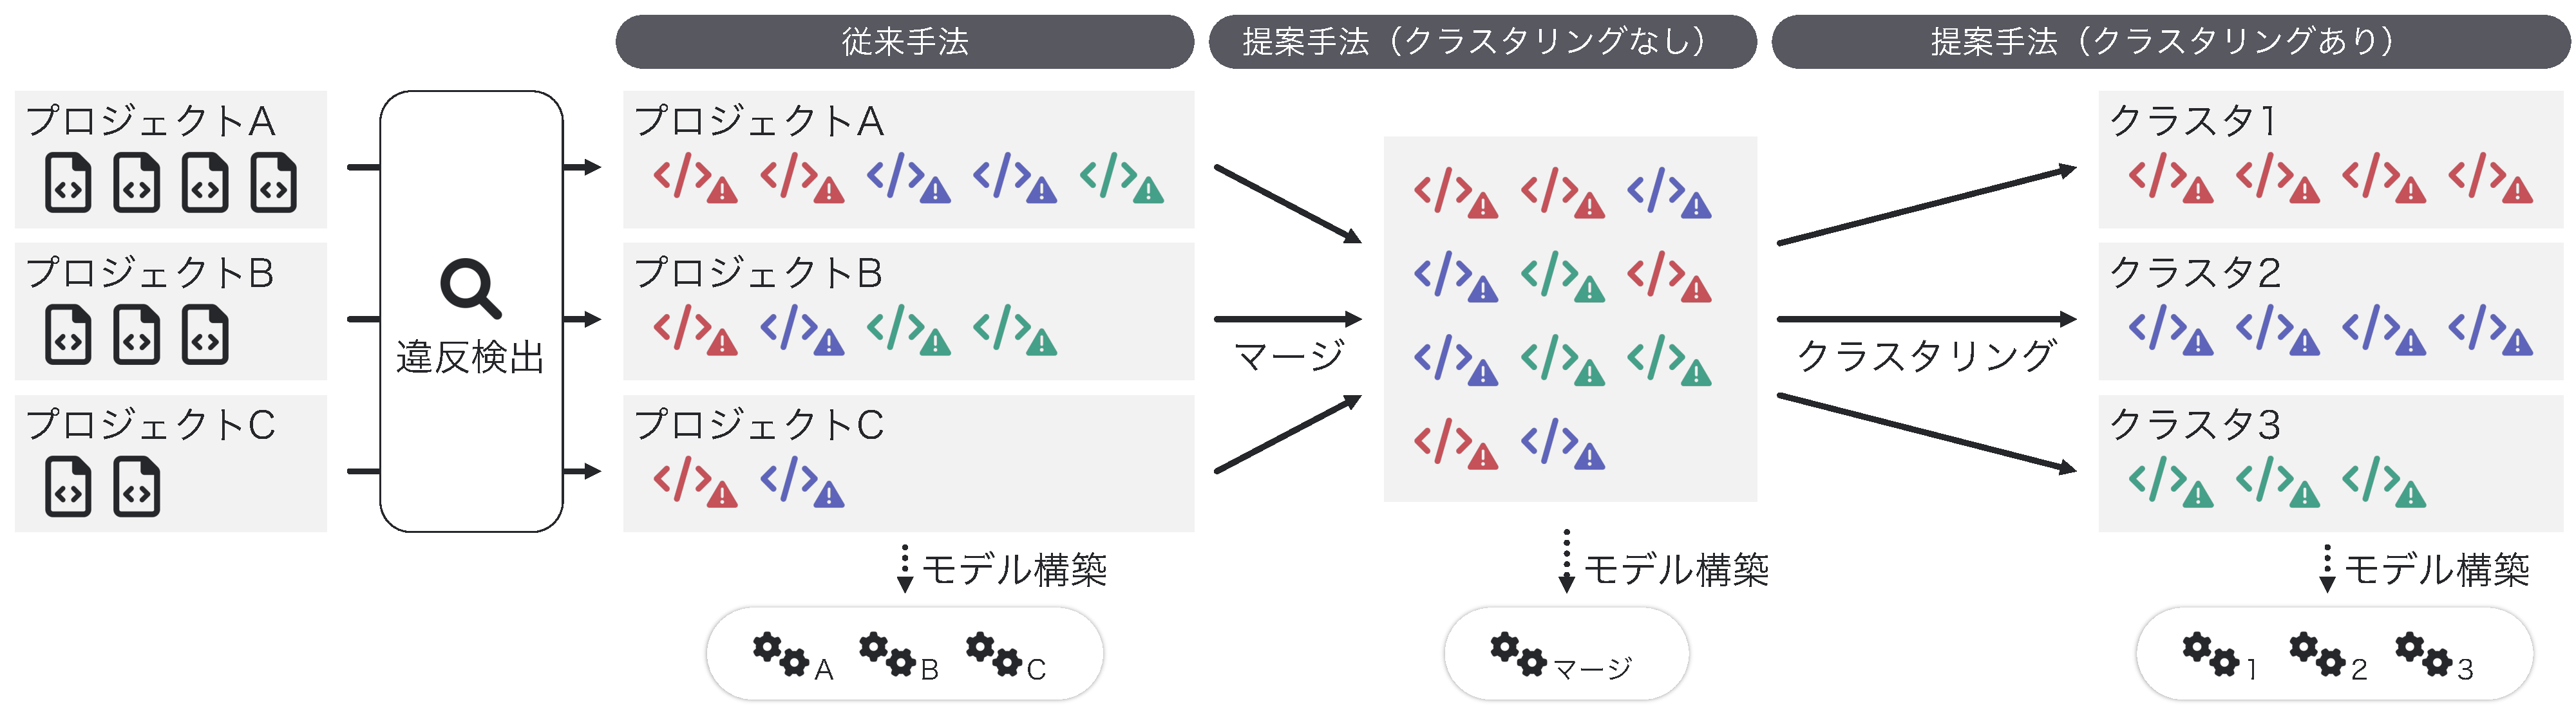
\includegraphics[width=1.0\linewidth]{Kameoka_fig/kameoka_fig1.pdf}
	\caption{本研究の概略図}
	\label{fig:Teiannsyuhou}
\end{figure*}

図\ref{fig:Teiannsyuhou}は本研究の検証手法を示す.本研究では,静的解析ツールによって検出されたコーディング規約違反を修正すべき違反かそうでない違反かの2値に分類する機械学習モデルを3種類作成する.各モデルの概要は以下の通りである.

\begin{enumerate}
  \item 従来研究の手法を採用したモデルであり,予測対象のプロジェクトの過去の規約修正履歴のみを学習する予測モデルを構築
  \item 提案手法の複数プロジェクトの規約修正履歴を学習させる手法で,すべての学習データを結合し学習する予測モデルを構築
  \item 提案手法で複数プロジェクトのデータを結合した後に,クラスタリングを行い各クラスタごとに学習する予測モデルを構築
\end{enumerate}

従来手法1種類と提案手法2種類の予測モデルを作成し,修正の要否を予測するモデルを評価する.評価の結果を基に,静的解析ツールの違反検出結果から修正要否の予測に対する本研究の有効性を検証する.

提案手法において,複数プロジェクトのデータを学習させる理由は,従来研究では,予測対象のプロジェクトと同プロジェクトの過去のデータを学習しているが,規約修正履歴がない場合や,違反回数が少ない場合に学習不足,または学習不可になることが発生する.この問題を解決するために,予測対象のプロジェクト以外のデータを学習させることによって学習データを補完する.

次に結合したデータをクラスタリングする理由を説明する.提案手法(クラスタリングなし)では,学習データに複数プロジェクトのデータを用いることによって学習データを拡張しており,各プロジェクトごとに存在するコーディングスタイルなどの特徴を無視したまま結合している.
% この問題に対してすべての違反修正履歴を
クラスタリングすることによって,説明変数が類似した違反修正データ群を収集することができるため,すべてのコーディング規約違反修正データを学習するより,類似性を持った説明変数から学習することができる.
クラスタリングによって説明変数が類似し同じクラスタに分類されたプロジェクト同士が,コーディングスタイルも類似するとは言えないが,説明変数同士の類似性を見ることによって,単純に結合した場合より効果的に複数プロジェクトのデータを学習できると考えられるため,クラスタリングを用いた手法を採用した.




%-----------------------------------prev
% 図\ref{fig:Teiannsyuhou}は,本研究の提案手法の概略図を示す.本研究では,規約に違反している箇所を修正するか否かを予測する3つの機械学習モデルを構築する.まず,図の左から,各プロジェクトのソースコードを対象に静的解析を行い,規約違反を含むソースコードの特徴量の計測,および,規約違反の修正有無を計測する.次に,学習データとして各プロジェクトの規約修正履歴のみを用いて機械学習モデル(従来手法)を構築する.続いて,各プロジェクトの規約修正履歴をすべて統合した学習データを用いた機械学習モデル(提案手法(クラスタリングなし))を構築する.最後に統合した学習データを階層的クラスタリングによって10クラスタに分割し,それぞれのクラスタの規約修正履歴を用いて機械学習モデル(提案手法(クラスタリングあり))を構築する.本研究では,評価に用いるオープンソースソフトウェアの対象プロジェクト数に合わせてクラスタ数を10としている.また,提案手法のクラスタリングは,全てのプロジェクトの学習データと評価用データを合わせてクラスタリングを行い,評価用データは,分類されたクラスタの学習データで構築したモデルを用いて予測する.
%-----------------------------------

\section{学習データと評価データの収集}

本研究では,複数プロジェクトのデータを学習するにあたって,すべてのプロジェクトのデータを学習に用いるために,各プロジェクトのデータを時系列順に並べた際の古いものから8割を学習に用い,残りの2割を検証用データとして用いた.ここで時系列順に並べている理由は,学習時に本来得られない未来のデータを学習させないために時系列の古いものを学習データとしている.そのため,モデルの評価時に,交差検証は行なわない.時系列を考慮した時系列十分割交差検証という手法も存在するが,データサイズが小さいプロジェクトでは,学習データサイズが小さくなりすぎることが危惧されるため,時系列十分割交差検証も行わない.

%-----------------------------------prev
% 本研究では,2種類の提案手法において構築する機械学習モデルにおいて複数のプロジェクトの規約修正履歴を統合するが,モデル構築に使用する学習データにも,検証に使用する評価データにも全てのプロジェクトが含まれるように考慮する.具体的には,各プロジェクトの分析対象期間に発生するコミットのうち,前半8割を学習データ,後半2割を評価データとし,各プロジェクトにおいて未来のデータを含まないようにするため交差検証を行わない.
%-----------------------------------




\section{説明変数・目的変数の計測方法}


%-------------------------
\begin{figure}[t]
	\centering
	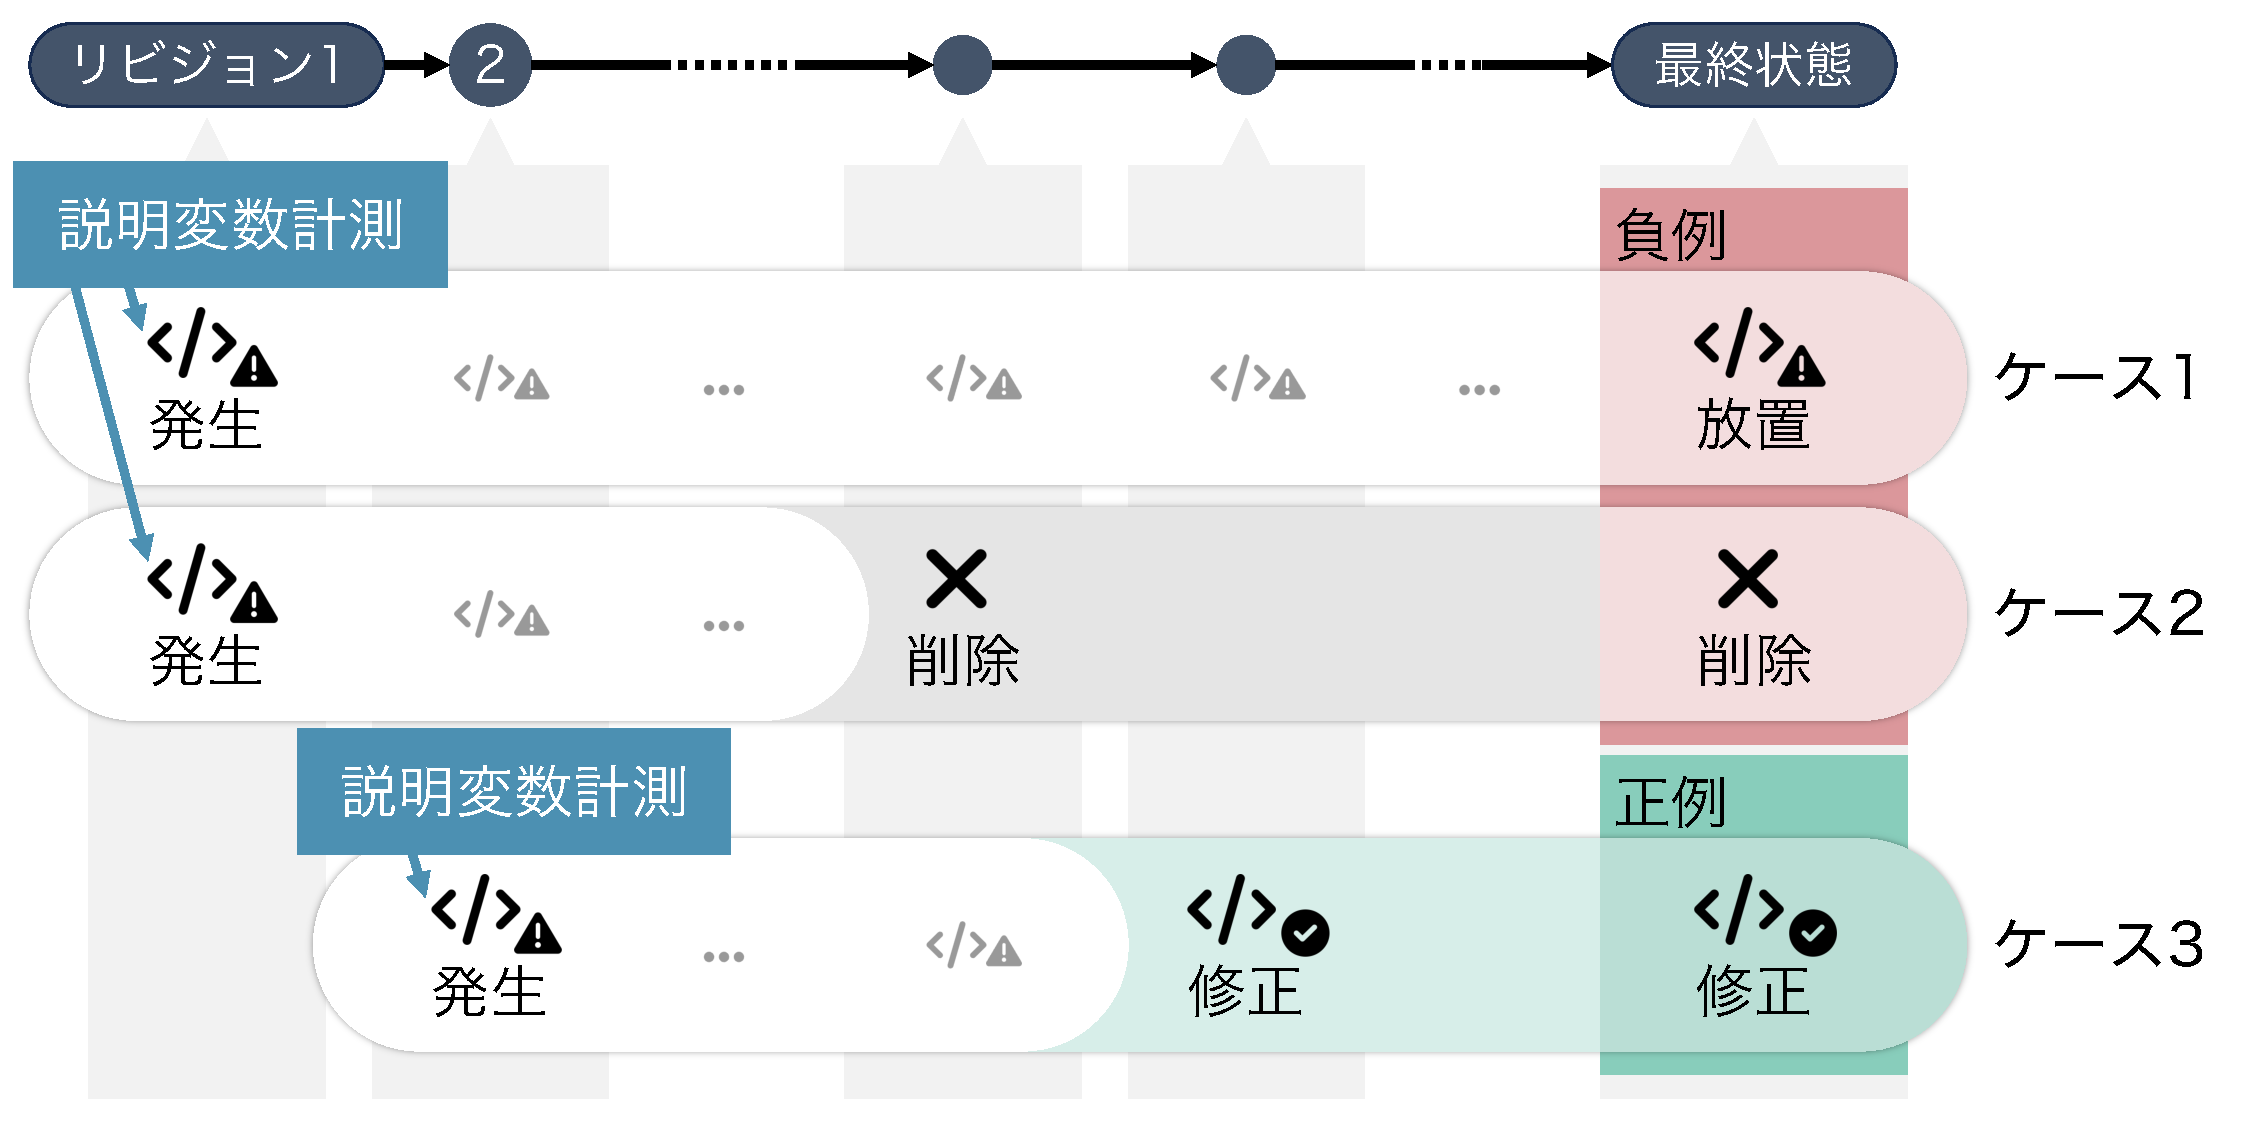
\includegraphics[width=1.0\linewidth]{Kameoka_fig/kameoka_fig2.pdf}
	\caption{説明変数と目的変数の計測方法}
	\label{fig:mokutekihensu}
\end{figure}
%-------------------------

図\ref{fig:mokutekihensu}は,本研究における説明変数と目的変数の計測位置と,計測方法を示す.本研究では,規約修正履歴から静的解析ツールによって初めて違反が検出された場所を説明変数の計測地点とし,最終状態において,各違反が修正されたか否かを計測することによって目的変数を計測する.
目的変数の計測についてケースごとにまとめたものが表\ref{tab:pos_neg}である.
図\ref{fig:mokutekihensu}と表\ref{tab:pos_neg}に示すケース1 - ケース3は各数字ごとに同じケースを示している.
各ケースについて詳しく説明すると,ケース1は,リビジョン1で発生した違反が修正されずに最終リビジョンまで放置された状況を表している.ケース2の事例は,発生した違反が途中状態で削除された場合を示している,最初の事例と2つ目の事例は発生した規約違反が修正されていないため負例として計測する.ケース3は,発生した違反が途中状態において修正された場合を示しており,最終状態において正例として計測する.説明変数はコーディング規約に違反するコード断片を含むソースコードファイルの関数,クラス,モジュールに対して特徴量をテクマトリックス株式会社が開発する静的解析ツールUnderstand\footnote{Understand: \url{https://www.techmatrix.co.jp/product/understand/}}を用いて計測する.

すべての計測したコーディング規約違反は表の3種類に分類され,目的変数を計測し,各違反の発生地点において説明変数を計測する.説明変数には,ソースコードの特徴量であるコード行数,コメント行数,循環的複雑度,コメント行数など含むソースコードに関する特徴量43種類に,コーディング規約違反IDをOne-hotベクトル化した1種類の,合計44種類の特徴量を使用する.


%-----------------------------------prev
% 本研究では,分析対象期間中のコミットにおいて変更されたPython言語で記述されたソースコード全てに静的解析ツールを実行する.特定のソースコード断片において初めて規約違反が検出されたコミットを,修正を要するか否かを判定する予測時点とし,説明変数を計測する.

% 図\ref{fig:mokutekihensu}は,説明変数と目的変数の計測事例を示す.この例では,コーディング規約への違反が3箇所で検出され,上2つはリビジョン1で発生し,下の1つはリビジョン2で発生しており,それぞれのリビジョンにおいて説明変数を計測する.説明変数の計測地点において,コーディング規約に違反するコード断片を含むソースコードファイルの関数,クラス,モジュールに対して特徴量をテクマトリックス株式会社が開発する静的解析ツールUnderstand\footnote{Understand: \url{https://www.techmatrix.co.jp/product/understand/}}を用いて計測する.説明変数は,ソースコードの特徴量であるコード行数,コメント行数,循環的複雑度,ネストの深さの最大値など含むソースコードに関する特徴量43種類に,コーディング規約の違反検出時に得られる違反箇所のコード行数1種類,規約違反IDをOne-hotベクトル化した1種類の,合計45種類の特徴量を使用する.
%-----------------------------------




% \section{目的変数の計測方法}

% 本研究では,分析対象期間中に修正されるか否かを目的変数とする.分析対象期間中に修正された規約違反のコード断片と修正されないままの規約違反含むコード断片は表\ref{tab:pos_neg}に示すように正例と負例の2クラスに分類する.

%----------------------
\begin{table}[t]
    \centering
    \caption{正例と負例の分類}
    \label{tab:pos_neg}
    \scalebox{1}{
    \begin{tabular}{l|l}
         \hline
            分類 & 説明\\ \hline
            負例(ケース1) & コーディング規約の違反が放置されているコード断片\\
            負例(ケース2) & コーディング規約に違反していたコード断片が削除された\\
            正例(ケース3) & コーディング規約に違反していたコード断片が修正された\\
         \hline
    \end{tabular}
    }
\end{table}
%-----------------------

\section{コーディング規約に違反しているコード断片のクラスタリング}


提案手法(クラスタリングあり)において,説明変数の特徴量が類似しているコード断片をクラスタリングし,各クラスタごとに予測モデルを構築する.クラスタリングには,クラスタ間の類似度を計測するため階層的クラスタリングを用いる.階層的クラスタリングには,連結法としてWard法を用い,距離の測定にはユークリッド距離を用いる\cite{ward}.本研究ではクラスタ数を10とした場合における結果を用いて評価を行う.クラスタ数を変化させることによって予測精度が変化することが考えられるが,本研究では予測結果についてい従来手法との差分を見たいため,クラスタ数を10のみの場合で検証している.

%-----------------------------------prev
% 本研究では,説明変数の特徴量が類似する規約違反しているコード断片をクラスタリングした後に,各クラスタに分類されたコード断片の学習データを用いてモデルを構築する.クラスタリングには,クラスタ間の類似度を確認するため階層的クラスタリングを用いる.階層的クラスタリングにおける,クラスタ間の距離はユークリッド距離を用い,クラスタの連結法にはWard法を用いる.本研究では検証に10プロジェクトの規約修正履歴を使用するため,クラスタ数を10とする.階層クラスタリングによって,従来手法で予測できなかったコード断片を分析する.
%-----------------------------------

\section{機械学習モデルの構築と評価}

本研究で利用する予測モデルは,機械学習の予測手法として頻繁に利用されるロジスティック回帰,RandomForest,SVMの3種類の手法を用いて予測モデルの構築を行う.
本研究で用いたデータセットに含まれるプロジェクトごとの違反修正率の中央値が0.36であるように,コーディング規約違反の修正に関するデータは,違反が修正された正例が少なく,修正されない負例が多い不均衡なデータであることが多いため,各予測モデルを構築するためのPythonパッケージに用意されているオプションであるclass\_weightsを用いることによって,2クラスデータに重みづけを行う.
また,学習の反復回数を定めるイテレーション回数を10,000に設定する.

構築した各予測モデルの評価には,従来研究でも用いられていた適合率,再現率,F1値を使用した.機械学習モデルの予測結果は以下の4種類に分類され,分類結果から各評価指標の値を算出する.

%-----------------------------------prev
% 予測モデルの構築には,
% Ruthruffらの従来研究と同様にロジスティック回帰モデルを用いる\cite{JyuraiPre}.本研究で取り扱うコーディング規約に違反しているコード断片は,修正されないままのコード断片が多数含まれる不均衡なデータとなっている.したがって,本研究ではロジスティック回帰分析にはPythonパッケージであるsklearnのlinear\_model.LogisticRegression\footnote{https://scikit-learn.org/stable/modules/generated/sklearn.linear\_model.LogisticRegression.html}を使用し,パッケージのオプションclass\_weightsを使用することで2クラスデータの分類に重み付けし,不均衡による問題を解決する.また,ロジスティック回帰モデルの学習を行う際にイテレーションの最大値を10,000回に設定する.

% 予測モデルの予測性能を評価する指標として,従来研究で用いられている適合率,再現率,F1値を使用する.機械学習モデルの予測結果は次の4つに分類することができ,分類結果に基づき各評価指標を算出する.
%-----------------------------------prev

\begin{itemize}
\item True Positive(TP): 修正された規約違反に対して,修正されると正しく予測するケース
\item False Positive(FP): 放置された規約違反に対して,修正されると誤って予測するケース
\item True Negative(TN):放置された規約違反に対して,放置されると正しく予測するケース
\item False Negative(FN):修正された規約違反に対して,放置されると誤って予測するケース
\end{itemize}

本研究における適合率は,修正予測モデルによって修正されると予測されたコーディング規約違反の内,実際に修正されたコーディング規約違反の割合を示す.再現率は実際に修正された違反の内,予測モデルによって予測できたものの割合を示す.F1値は適合率と再現率を用いて式\ref{f-measure}を用いて算出される適合率と再現率のトレードオフの関係に着目した評価指標である.

\begin{equation}
  F値 = \frac{2 * 適合率 * 再現率}{適合率 + 再現率} \label{f-measure}
\end{equation}

\chapter{評価実験}\label{chap:result}

\section{データセット}

\begin{figure}[tbp]
	\centering
	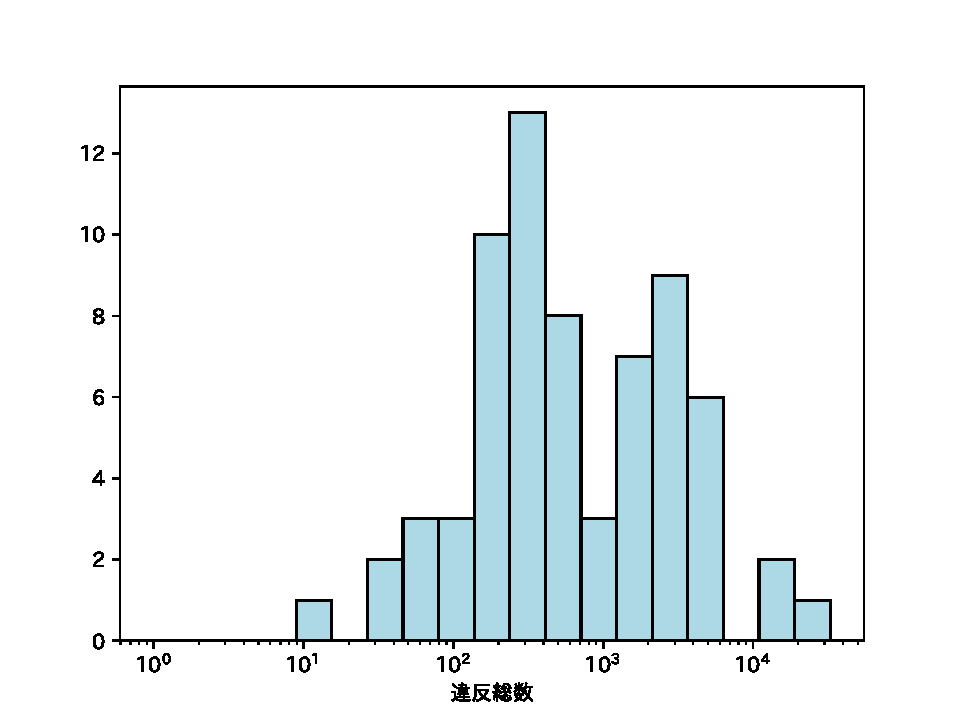
\includegraphics[width=0.7\linewidth]{Kameoka_fig/dataset_hist.pdf}
	\caption{データセットに含まれるプロジェクトごとの違反総数のヒストグラム}
	\label{fig:dataset}
\end{figure}

\subsection{対象プロジェクトの選定方法}
本研究ではケーススタディとして,OSSライブラリ検索サービスであるLibraries.io\footnote{Libraries.io: \url{https://libraries.io/}}からPython言語で実装され,静的解析ツールPylintを開発に使用しており,GitHubにソフトウェア,および規約修正履歴を公開しているプロジェクトを対象とする.
具体的には,Librsries.ioにおいてOSSの人気度合いや活発度合いを示すSourceRankの上位1,500プロジェクトから静的解析ツールの設定ファイル(pylintrc or .pylintrc)を保有する81プロジェクトの内,取得した目的変数を学習用データと検証用データに分割した際に,どちらのデータにも正例と負例を含む68プロジェクトを対象とする.

本研究では,各分析対象プロジェクトにおいて,2018年12月から1,000日間のコミット履歴を分析対象とする.図\ref{fig:dataset}に,各プロジェクトの総コーディング規約違反数をヒストグラムで示す.図の横軸はプロジェクトごとの総違反数対数軸で示す.違反数が100-1,000のプロジェクトが最も多い.

\subsection{対象プログラミング言語の選定理由}

Python言語は,近年のLLM(大規模言語モデル)をはじめとする機械学習技術の開発・利用に頻繁に用いられている.また,Pythonはデータ分析においても充実したライブラリが存在し,その有用性が広く知られている.よって,本研究ではPython言語を対象言語として選択した.

\subsection{静的解析ツールの選定理由}

本研究で分析対象とする静的解析ツールにはPylintを選定した.Pylintは他の静的解析ツールより多くのコーディング規約が設定されていることが特徴である.Python言語のコーディング規約であるPEP8に基づいた静的解析ツールは数多く存在するが,Pylintは設定ファイルによるスタイルチェックや論理エラーチェックの対象を柔軟にカスタマイズすることができ,Pythonの代表的な静的解析ツールのflake8より厳しい判定基準を設けている.Pylintのコーディング規約は次の6カテゴリに分類されている.

\begin{itemize}
  \item F (Fatal)カテゴリ
  \item E (Error)カテゴリ
  \item W (Warning)カテゴリ
  \item C (Convention)カテゴリ
  \item R (Refactor)カテゴリ
  \item I (Information)カテゴリ
\end{itemize}

このうちFカテゴリとIカテゴリはPylintそのものや設定ファイルに関するエラーを検出した際のエラーカテゴリであるため,実際のソースコードにPylintを適用した際にはE, W, C, Rの4カテゴリーのコーディング規約違反が検出する.Pylintは他の静的解析ツールより豊富なルールでコーディング規約違反を検出することができ,ソースコードから4カテゴリに分類される多くの違反を検出できるため本研究での対象静的解析ツールとして選択した.

\section{RQ1: 複数プロジェクトのデータ用いることで予測精度は向上するか?}

\subsection{実験結果}

\begin{table}{}
    \centering
    \caption{各手法による評価指標で最も高い値で予測したプロジェクト数の一覧}
    \label{tab:gen}
    \vspace{3mm}
    \scalebox{0.75}{
        \begin{tabular}{l|p{7em}p{7em}p{7em}|p{7em}p{7em}p{7em}|p{7em}p{7em}p{7em}}
            \hline
            \multirow{2}{*}{手法}&\multicolumn{3}{c|}{{ロジスティック回帰}} & \multicolumn{3}{c|}{RandomForest} & \multicolumn{3}{c}{SVM}\\ \cline{2-10}
             & \multicolumn{1}{r}{{適合率}} & \multicolumn{1}{r}{{再現率}} & \multicolumn{1}{r|}{{F1値}} & \multicolumn{1}{r}{{適合率}} & \multicolumn{1}{r}{{再現率}} & \multicolumn{1}{r|}{{F1値}} & \multicolumn{1}{r}{{適合率}} & \multicolumn{1}{r}{{再現率}} & \multicolumn{1}{r}{{F1値}}\\ \hline
            従来手法 & \multicolumn{1}{r}{{48}} & \multicolumn{1}{r}{{27}} & \multicolumn{1}{r|}{{38}} & \multicolumn{1}{r}{{28}} & \multicolumn{1}{r}{{43}} & \multicolumn{1}{r|}{{37}} & \multicolumn{1}{r}{{36}} & \multicolumn{1}{r}{{24}} & \multicolumn{1}{r}{{28}} \\
            % 提案手法(クラスタリングなし) & 12 & 40 & 18 & 27 & 35 & 23 & 17 & 25 & 18 \\
            提案手法(クラスタリングなし) & \multicolumn{1}{r}{{12}} & \multicolumn{1}{r}{{40}} & \multicolumn{1}{r|}{{18}} & \multicolumn{1}{r}{{27}} & \multicolumn{1}{r}{{35}} & \multicolumn{1}{r|}{{23}} & \multicolumn{1}{r}{{17}} & \multicolumn{1}{r}{{25}} & \multicolumn{1}{r}{{18}} \\
            % 提案手法(クラスタリングあり) & 20 & 22 & 19  & 28 & 24 & 16 & 24 & 36 & 26 \\ \hline
            提案手法(クラスタリングあり) & \multicolumn{1}{r}{{20}} & \multicolumn{1}{r}{{22}} & \multicolumn{1}{r|}{{19}}  & \multicolumn{1}{r}{{28}} & \multicolumn{1}{r}{{24}} & \multicolumn{1}{r|}{{16}} & \multicolumn{1}{r}{{24}} & \multicolumn{1}{r}{{36}} & \multicolumn{1}{r}{{26}} \\ \hline
            % 重複数 & 12 & 21 & 7 & 15 & 34 & 8 & 9 & 17 & 4 \\ \hline
            重複数 & \multicolumn{1}{r}{{12}} & \multicolumn{1}{r}{{21}} & \multicolumn{1}{r|}{{7}} & \multicolumn{1}{r}{{15}} & \multicolumn{1}{r}{{34}} & \multicolumn{1}{r|}{{8}} & \multicolumn{1}{r}{{9}} & \multicolumn{1}{r}{{17}} & \multicolumn{1}{r}{{4}} \\ \hline
        \end{tabular}
    }
\end{table}

\begin{table}{}
    \centering
    \caption{ロジスティック回帰モデルでの予測結果(総違反数の上下5件ずつを掲載)}
    \label{tab:logistic}
    \vspace{3mm}
    \scalebox{0.75}{
        \begin{tabular}{l||p{4em}|p{4em}|p{4em}||p{4em}|p{4em}|p{4em}||p{4em}|p{4em}|p{4em}}
            \hline
            \multirow{3}{*}{プロジェクト名}&\multicolumn{3}{c||}{\multirow{2}{*}{従来手法}} & \multicolumn{3}{c||}{提案手法} & \multicolumn{3}{c}{提案手法}\\
            &\multicolumn{3}{c||}{} & \multicolumn{3}{c||}{(クラスタリングなし)} & \multicolumn{3}{c}{(クラスタリングあり)}\\ \cline{2-10}
            & 適合率 & 再現率 & F1値 & 適合率 & 再現率 & F1値 & 適合率 & 再現率 & F1値 \\ \hline
            sockeye & \multicolumn{1}{r|}{\textbf{0.53}} & \multicolumn{1}{r|}{\textbf{0.81}} & \multicolumn{1}{r||}{\textbf{0.64}} & \multicolumn{1}{r|}{0.35} & \multicolumn{1}{r|}{0.56} & \multicolumn{1}{r||}{0.43} & \multicolumn{1}{r|}{0.49} & \multicolumn{1}{r|}{0.67} & \multicolumn{1}{r}{0.57} \\
            coretools & \multicolumn{1}{r|}{\textbf{0.04}} & \multicolumn{1}{r|}{0.63} & \multicolumn{1}{r||}{\textbf{0.07}} & \multicolumn{1}{r|}{0.02} & \multicolumn{1}{r|}{\textbf{0.88}} & \multicolumn{1}{r||}{0.04} & \multicolumn{1}{r|}{0.03} & \multicolumn{1}{r|}{0.83} & \multicolumn{1}{r}{0.05} \\
            howdoi & \multicolumn{1}{r|}{\textbf{0.64}} & \multicolumn{1}{r|}{\textbf{0.99}} & \multicolumn{1}{r||}{\textbf{0.78}} & \multicolumn{1}{r|}{0.12} & \multicolumn{1}{r|}{0.33} & \multicolumn{1}{r||}{0.17} & \multicolumn{1}{r|}{0.22} & \multicolumn{1}{r|}{0.25} & \multicolumn{1}{r}{0.23} \\
            schema\_salad & \multicolumn{1}{r|}{\textbf{0.55}} & \multicolumn{1}{r|}{0.27} & \multicolumn{1}{r||}{0.37} & \multicolumn{1}{r|}{0.51} & \multicolumn{1}{r|}{\textbf{0.64}} & \multicolumn{1}{r||}{\textbf{0.56}} & \multicolumn{1}{r|}{\textbf{0.55}} & \multicolumn{1}{r|}{0.54} & \multicolumn{1}{r}{0.54} \\
            serverless-application-model & \multicolumn{1}{r|}{\textbf{0.76}} & \multicolumn{1}{r|}{0.45} & \multicolumn{1}{r||}{0.57} & \multicolumn{1}{r|}{0.55} & \multicolumn{1}{r|}{\textbf{0.83}} & \multicolumn{1}{r||}{0.66} & \multicolumn{1}{r|}{0.64} & \multicolumn{1}{r|}{\textbf{0.83}} & \multicolumn{1}{r}{\textbf{0.72}} \\
            \hline \hline
            implicit & \multicolumn{1}{r|}{\textbf{1.00}} & \multicolumn{1}{r|}{0.44} & \multicolumn{1}{r||}{0.62} & \multicolumn{1}{r|}{0.70} & \multicolumn{1}{r|}{\textbf{0.78}} & \multicolumn{1}{r||}{\textbf{0.74}} & \multicolumn{1}{r|}{\textbf{1.00}} & \multicolumn{1}{r|}{0.11} & \multicolumn{1}{r}{0.20} \\
            python-sshpubkeys & \multicolumn{1}{r|}{0.64} & \multicolumn{1}{r|}{\textbf{1.00}} & \multicolumn{1}{r||}{\textbf{0.78}} & \multicolumn{1}{r|}{\textbf{0.71}} & \multicolumn{1}{r|}{0.71} & \multicolumn{1}{r||}{0.71} & \multicolumn{1}{r|}{0.64} & \multicolumn{1}{r|}{\textbf{1.00}} & \multicolumn{1}{r}{\textbf{0.78}} \\
            munch & \multicolumn{1}{r|}{\textbf{0.43}} & \multicolumn{1}{r|}{\textbf{1.00}} & \multicolumn{1}{r||}{\textbf{0.60}} & \multicolumn{1}{r|}{0.33} & \multicolumn{1}{r|}{0.33} & \multicolumn{1}{r||}{0.33} & \multicolumn{1}{r|}{0.38} & \multicolumn{1}{r|}{\textbf{1.00}} & \multicolumn{1}{r}{0.55} \\
            python-resize-image & \multicolumn{1}{r|}{0.14} & \multicolumn{1}{r|}{\textbf{1.00}} & \multicolumn{1}{r||}{0.25} & \multicolumn{1}{r|}{0.17} & \multicolumn{1}{r|}{\textbf{1.00}} & \multicolumn{1}{r||}{0.29} & \multicolumn{1}{r|}{\textbf{0.20}} & \multicolumn{1}{r|}{\textbf{1.00}} & \multicolumn{1}{r}{\textbf{0.33}} \\
            queuelib & \multicolumn{1}{r|}{nan} & \multicolumn{1}{r|}{0.00} & \multicolumn{1}{r||}{nan} & \multicolumn{1}{r|}{\textbf{0.33}} & \multicolumn{1}{r|}{\textbf{1.00}} & \multicolumn{1}{r||}{\textbf{0.50}} & \multicolumn{1}{r|}{\textbf{0.33}} & \multicolumn{1}{r|}{\textbf{1.00}} & \multicolumn{1}{r}{\textbf{0.50}} \\ \hline
        \end{tabular}
    }
\end{table}

\begin{table}{}
    \centering
    \caption{RandomForestモデルでの予測結果(総違反数の上下5件ずつを掲載)}
    \label{tab:RandomForest}
    \vspace{3mm}
    \scalebox{0.75}{
        \begin{tabular}{l||p{4em}|p{4em}|p{4em}||p{4em}|p{4em}|p{4em}||p{4em}|p{4em}|p{4em}}
            \hline
            \multirow{3}{*}{プロジェクト名}&\multicolumn{3}{c||}{\multirow{2}{*}{従来手法}} & \multicolumn{3}{c||}{提案手法} & \multicolumn{3}{c}{提案手法}\\
            &\multicolumn{3}{c||}{} & \multicolumn{3}{c||}{(クラスタリングなし)} & \multicolumn{3}{c}{(クラスタリングあり)}\\ \cline{2-10}
            & 適合率 & 再現率 & F1値 & 適合率 & 再現率 & F1値 & 適合率 & 再現率 & F1値 \\ \hline
            sockeye & \multicolumn{1}{r|}{0.75} & \multicolumn{1}{r|}{\textbf{0.83}} & \multicolumn{1}{r||}{\textbf{0.79}} & \multicolumn{1}{r|}{\textbf{0.76}} & \multicolumn{1}{r|}{0.79} & \multicolumn{1}{r||}{0.78} & \multicolumn{1}{r|}{\textbf{0.76}} & \multicolumn{1}{r|}{0.80} & \multicolumn{1}{r}{0.78} \\
            coretools & \multicolumn{1}{r|}{\textbf{0.14}} & \multicolumn{1}{r|}{0.24} & \multicolumn{1}{r||}{\textbf{0.18}} & \multicolumn{1}{r|}{0.04} & \multicolumn{1}{r|}{\textbf{0.41}} & \multicolumn{1}{r||}{0.08} & \multicolumn{1}{r|}{0.04} & \multicolumn{1}{r|}{0.37} & \multicolumn{1}{r}{0.07} \\
            howdoi & \multicolumn{1}{r|}{\textbf{0.78}} & \multicolumn{1}{r|}{\textbf{0.99}} & \multicolumn{1}{r||}{\textbf{0.87}} & \multicolumn{1}{r|}{0.07} & \multicolumn{1}{r|}{\textbf{0.99}} & \multicolumn{1}{r||}{0.13} & \multicolumn{1}{r|}{0.07} & \multicolumn{1}{r|}{\textbf{0.99}} & \multicolumn{1}{r}{0.13} \\
            schema\_salad & \multicolumn{1}{r|}{\textbf{0.66}} & \multicolumn{1}{r|}{\textbf{0.58}} & \multicolumn{1}{r||}{\textbf{0.62}} & \multicolumn{1}{r|}{0.58} & \multicolumn{1}{r|}{0.31} & \multicolumn{1}{r||}{0.41} & \multicolumn{1}{r|}{0.46} & \multicolumn{1}{r|}{0.21} & \multicolumn{1}{r}{0.29} \\
            serverless-application-model & \multicolumn{1}{r|}{\textbf{0.72}} & \multicolumn{1}{r|}{\textbf{0.27}} & \multicolumn{1}{r||}{\textbf{0.39}} & \multicolumn{1}{r|}{0.70} & \multicolumn{1}{r|}{0.23} & \multicolumn{1}{r||}{0.34} & \multicolumn{1}{r|}{0.63} & \multicolumn{1}{r|}{0.24} & \multicolumn{1}{r}{0.35} \\
            \hline \hline
            implicit & \multicolumn{1}{r|}{0.75} & \multicolumn{1}{r|}{\textbf{1.00}} & \multicolumn{1}{r||}{\textbf{0.86}} & \multicolumn{1}{r|}{\textbf{1.00}} & \multicolumn{1}{r|}{0.44} & \multicolumn{1}{r||}{0.62} & \multicolumn{1}{r|}{\textbf{1.00}} & \multicolumn{1}{r|}{0.44} & \multicolumn{1}{r}{0.62} \\
            python-sshpubkeys & \multicolumn{1}{r|}{0.64} & \multicolumn{1}{r|}{\textbf{1.00}} & \multicolumn{1}{r||}{\textbf{0.78}} & \multicolumn{1}{r|}{\textbf{0.71}} & \multicolumn{1}{r|}{0.71} & \multicolumn{1}{r||}{0.71} & \multicolumn{1}{r|}{0.67} & \multicolumn{1}{r|}{0.29} & \multicolumn{1}{r}{0.40} \\
            munch & \multicolumn{1}{r|}{nan} & \multicolumn{1}{r|}{0.00} & \multicolumn{1}{r||}{nan} & \multicolumn{1}{r|}{nan} & \multicolumn{1}{r|}{0.00} & \multicolumn{1}{r||}{nan} & \multicolumn{1}{r|}{nan} & \multicolumn{1}{r|}{0.00} & \multicolumn{1}{r}{nan} \\
            python-resize-image & \multicolumn{1}{r|}{0.14} & \multicolumn{1}{r|}{\textbf{1.00}} & \multicolumn{1}{r||}{0.25} & \multicolumn{1}{r|}{0.14} & \multicolumn{1}{r|}{\textbf{1.00}} & \multicolumn{1}{r||}{0.25} & \multicolumn{1}{r|}{\textbf{0.17}} & \multicolumn{1}{r|}{\textbf{1.00}} & \multicolumn{1}{r}{\textbf{0.29}} \\
            queuelib & \multicolumn{1}{r|}{nan} & \multicolumn{1}{r|}{0.00} & \multicolumn{1}{r||}{nan} & \multicolumn{1}{r|}{nan} & \multicolumn{1}{r|}{0.00} & \multicolumn{1}{r||}{nan} & \multicolumn{1}{r|}{nan} & \multicolumn{1}{r|}{0.00} & \multicolumn{1}{r}{nan} \\ \hline
        \end{tabular}
    }
\end{table}

\begin{table}{}
    \centering
    \caption{SVMモデルでの予測結果(総違反数の上下5件ずつを掲載)}
    \label{tab:SVM}
    \vspace{3mm}
    \scalebox{0.75}{
        \begin{tabular}{l||p{4em}|p{4em}|p{4em}||p{4em}|p{4em}|p{4em}||p{4em}|p{4em}|p{4em}}
            \hline
            \multirow{3}{*}{プロジェクト名}&\multicolumn{3}{c||}{\multirow{2}{*}{従来手法}} & \multicolumn{3}{c||}{提案手法} & \multicolumn{3}{c}{提案手法}\\
            &\multicolumn{3}{c||}{} & \multicolumn{3}{c||}{(クラスタリングなし)} & \multicolumn{3}{c}{(クラスタリングあり)}\\ \cline{2-10}
            & 適合率 & 再現率 & F1値 & 適合率 & 再現率 & F1値 & 適合率 & 再現率 & F1値 \\ \hline
            sockeye & \multicolumn{1}{r|}{0.47} & \multicolumn{1}{r|}{\textbf{0.71}} & \multicolumn{1}{r||}{\textbf{0.57}} & \multicolumn{1}{r|}{0.30} & \multicolumn{1}{r|}{0.48} & \multicolumn{1}{r||}{0.37} & \multicolumn{1}{r|}{\textbf{0.50}} & \multicolumn{1}{r|}{0.60} & \multicolumn{1}{r}{0.54} \\
            coretools & \multicolumn{1}{r|}{0.02} & \multicolumn{1}{r|}{0.68} & \multicolumn{1}{r||}{0.04} & \multicolumn{1}{r|}{0.02} & \multicolumn{1}{r|}{0.49} & \multicolumn{1}{r||}{0.03} & \multicolumn{1}{r|}{\textbf{0.03}} & \multicolumn{1}{r|}{\textbf{0.88}} & \multicolumn{1}{r}{\textbf{0.06}} \\
            howdoi & \multicolumn{1}{r|}{0.05} & \multicolumn{1}{r|}{\textbf{0.99}} & \multicolumn{1}{r||}{0.10} & \multicolumn{1}{r|}{0.05} & \multicolumn{1}{r|}{0.21} & \multicolumn{1}{r||}{0.08} & \multicolumn{1}{r|}{\textbf{0.15}} & \multicolumn{1}{r|}{0.20} & \multicolumn{1}{r}{\textbf{0.17}} \\
            schema\_salad & \multicolumn{1}{r|}{0.48} & \multicolumn{1}{r|}{0.43} & \multicolumn{1}{r||}{0.45} & \multicolumn{1}{r|}{\textbf{0.51}} & \multicolumn{1}{r|}{0.58} & \multicolumn{1}{r||}{0.54} & \multicolumn{1}{r|}{\textbf{0.51}} & \multicolumn{1}{r|}{\textbf{0.66}} & \multicolumn{1}{r}{\textbf{0.57}} \\
            serverless-application-model & \multicolumn{1}{r|}{\textbf{0.69}} & \multicolumn{1}{r|}{0.56} & \multicolumn{1}{r||}{0.62} & \multicolumn{1}{r|}{0.47} & \multicolumn{1}{r|}{0.37} & \multicolumn{1}{r||}{0.41} & \multicolumn{1}{r|}{0.59} & \multicolumn{1}{r|}{\textbf{0.77}} & \multicolumn{1}{r}{\textbf{0.67}} \\
            \hline \hline
            implicit & \multicolumn{1}{r|}{\textbf{1.00}} & \multicolumn{1}{r|}{\textbf{0.44}} & \multicolumn{1}{r||}{\textbf{0.62}} & \multicolumn{1}{r|}{0.57} & \multicolumn{1}{r|}{\textbf{0.44}} & \multicolumn{1}{r||}{0.50} & \multicolumn{1}{r|}{\textbf{1.00}} & \multicolumn{1}{r|}{0.22} & \multicolumn{1}{r}{0.36} \\
            python-sshpubkeys & \multicolumn{1}{r|}{\textbf{0.64}} & \multicolumn{1}{r|}{\textbf{1.00}} & \multicolumn{1}{r||}{\textbf{0.78}} & \multicolumn{1}{r|}{nan} & \multicolumn{1}{r|}{0.00} & \multicolumn{1}{r||}{nan} & \multicolumn{1}{r|}{\textbf{0.64}} & \multicolumn{1}{r|}{\textbf{1.00}} & \multicolumn{1}{r}{\textbf{0.78}} \\
            munch & \multicolumn{1}{r|}{nan} & \multicolumn{1}{r|}{0.00} & \multicolumn{1}{r||}{nan} & \multicolumn{1}{r|}{\textbf{1.00}} & \multicolumn{1}{r|}{\textbf{0.33}} & \multicolumn{1}{r||}{\textbf{0.50}} & \multicolumn{1}{r|}{\textbf{1.00}} & \multicolumn{1}{r|}{\textbf{0.33}} & \multicolumn{1}{r}{\textbf{0.50}} \\
            python-resize-image & \multicolumn{1}{r|}{0.14} & \multicolumn{1}{r|}{\textbf{1.00}} & \multicolumn{1}{r||}{0.25} & \multicolumn{1}{r|}{\textbf{0.50}} & \multicolumn{1}{r|}{\textbf{1.00}} & \multicolumn{1}{r||}{\textbf{0.67}} & \multicolumn{1}{r|}{0.20} & \multicolumn{1}{r|}{\textbf{1.00}} &\multicolumn{1}{r}{0.33} \\
            queuelib & \multicolumn{1}{r|}{nan} & \multicolumn{1}{r|}{0.00} & \multicolumn{1}{r||}{nan} & \multicolumn{1}{r|}{nan} & \multicolumn{1}{r|}{0.00} & \multicolumn{1}{r||}{nan} & \multicolumn{1}{r|}{\textbf{0.33}} & \multicolumn{1}{r|}{\textbf{1.00}} & \multicolumn{1}{r}{\textbf{0.50}} \\ \hline
        \end{tabular}
    }
\end{table}

\begin{table}{}
    \centering
    \caption{ロジスティック回帰モデルで再現率とF1値が顕著に変化した予測結果}
    \label{tab:log-super}
    \vspace{3mm}
    \scalebox{0.75}{
        \begin{tabular}{l|p{4em}p{4em}p{4em}|p{4em}p{4em}p{4em}|p{4em}p{4em}p{4em}}
            \hline
            \multirow{3}{*}{プロジェクト名}&\multicolumn{3}{c|}{\multirow{2}{*}{従来手法}} & \multicolumn{3}{c|}{提案手法} & \multicolumn{3}{c}{提案手法}\\
            &\multicolumn{3}{c|}{} & \multicolumn{3}{c|}{(クラスタリングなし)} & \multicolumn{3}{c}{(クラスタリングあり)}\\ \cline{2-10}
            & 適合率 & 再現率 & F1値 & 適合率 & 再現率 & F1値 & 適合率 & 再現率 & F1値 \\ \hline
            schema\_salad & \multicolumn{1}{r}{0.55} & \multicolumn{1}{r}{0.27} & \multicolumn{1}{r|}{0.37} & \multicolumn{1}{r}{0.51} & \multicolumn{1}{r}{0.64} & \multicolumn{1}{r|}{0.56} & \multicolumn{1}{r}{0.55} & \multicolumn{1}{r}{0.54} & \multicolumn{1}{r}{0.54} \\
            serverless-application-model & \multicolumn{1}{r}{0.76} & \multicolumn{1}{r}{0.45}& \multicolumn{1}{r|}{0.57} & \multicolumn{1}{r}{0.55} & \multicolumn{1}{r}{0.83} & \multicolumn{1}{r|}{0.66} & \multicolumn{1}{r}{0.64} & \multicolumn{1}{r}{0.83} & \multicolumn{1}{r}{0.72} \\
            transitions & \multicolumn{1}{r}{0.83} & \multicolumn{1}{r}{0.92} & \multicolumn{1}{r|}{0.87} & \multicolumn{1}{r}{0.67} & \multicolumn{1}{r}{0.61} & \multicolumn{1}{r|}{0.64} & \multicolumn{1}{r}{0.63} & \multicolumn{1}{r}{0.86} & \multicolumn{1}{r}{0.73} \\
            django-fsm & \multicolumn{1}{r}{0.62} & \multicolumn{1}{r}{0.99} & \multicolumn{1}{r|}{0.76} & \multicolumn{1}{r}{0.57} & \multicolumn{1}{r}{0.76} & \multicolumn{1}{r|}{0.65} & \multicolumn{1}{r}{0.60} & \multicolumn{1}{r}{0.76} & \multicolumn{1}{r}{0.67} \\ \hline
        \end{tabular}
    }
\end{table}


表\ref{tab:gen}は従来手法,提案手法(クラスタリングなし),提案手法(クラスタリングあり)の予測結果を評価した概要を示す.
表中の値は各手法において,適合率,再現率,F1値を算出し,最大値をとったプロジェクト数を記載している.
具体的には,ロジスティック回帰モデルの適合率は,従来手法の場合68プロジェクト中48プロジェクトが,提案手法(クラスタリングなし)では68プロジェクト中12プロジェクト,提案手法(クラスタリングあり)では68プロジェクト中20プロジェクトが他の手法以上の適合率で予測ができていることを示す.従来手法,提案手法(クラスタリングなし),提案手法(クラスタリングあり)の各指標のプロジェクト数の総和がデータセット全体の68プロジェクトを超えるのは,同じプロジェクトを重複してカウントしているからである.
重複数は,各プロジェクトの同じ指標で異なる手法において同じ値を取った場合,最大値をとったすべての手法でカウントしているため,同じプロジェクトが重複して数えられた回数を示している.各評価指標は有効数字2桁で算出し,予測の精度が各手法間で一致することもあるため,重複が発生している.

それぞれの手法とモデル構築手法のF1値を比較すると,従来手法が最多の最大値をとっていることがわかる.
しかし,提案手法によって再現率が改善されているプロジェクトが多い.
特にロジスティック回帰モデルの再現率が最大値のプロジェクト数は従来手法で27であり,提案手法(クラスタリングなし)では40に増加している.再現率が向上した理由として,提案手法は複数プロジェクトのデータを学習に用いているため,単一プロジェクトでは,修正が必要であることを学習できなかった違反を,学習データを拡張したことによって予測が可能になったと考えられる.
データセットを拡張したことによって,正例と予測する範囲が広がったため,従来手法で真陰性として予測できていたものを偽陽性として予測したため,提案手法によって適合率が低下したと考えられる.これについて\ref{kosatu}章で考察する.

表\ref{tab:logistic}から\ref{tab:SVM}は従来手法と提案手法2種の予測結果の値を示す.
各表はプロジェクトに対して従来手法,提案手法(クラスタリングなし),提案手法(クラスタリングあり)による予測結果の適合率,再現率,F1値を算出したものである.
結果として掲載しているプロジェクトは,各プロジェクトで検出された違反総数でソートした上位と下位から5プロジェクトを抽出したものである.
表\ref{tab:logistic}, \ref{tab:RandomForest}中に含まれる`nan'は予測結果をすべて負例として予測し,適合率とF1値を計算することができなかったため`nan'としている.
予測結果の再現率が向上したプロジェクトは,違反総数で降順にソートした場合,データ数が多い方から20プロジェクト目以降で頻繁に見られた.
表\ref{tab:logistic}から\ref{tab:SVM}を比較すると表\ref{tab:RandomForest} のRandomForestモデルの結果が最も高いF1値で予測できていることがわかる.また,表\ref{tab:SVM}のSVMモデルの結果が最もF1値が低い予測結果となっている.また,SVMモデルは提案手法(クラスタリングなし)のモデルを構築する際に本研究の実行環境では60時間を要した.よってSVMモデルは静的解析ツールによって検出されたコーディング規約違反の修正要否予測モデルには適していない.

\subsection{結果のまとめ}

最も予測精度の高かったRandomForestモデルの従来手法では全プロジェクトの半数程度の37プロジェクト,提案手法(クラスタリングなし)では23プロジェクト,提案手法(クラスタリングあり)では16プロジェクトでF1値の最大値をとっている.ロジスティック回帰モデルの場合,学習データが十分に集まるプロジェクトでは従来手法のような単一のプロジェクトの規約修正履歴を学習し,プロジェクトごとの修正の特性を考慮した予測を行う方が高い精度で修正予測ができ,そうでない場合は提案手法のように予測対象以外のプロジェクトの開発データを用いて学習することが効果的であることが示唆される.つまり,個々のプロジェクトでの総違反発生数が1,000以下の場合,ロジスティック回帰モデルでは提案手法によって予測精度が向上することが多い.

\section{RQ2: 提案手法によって従来手法では予測できなかった修正予測ができるのか?}\label{RQ2}

\subsection{実験結果}

% \begin{table}
%   \caption{分析に用いる混合行列のフォーマット} \label{tab:confusion_matrix}
%   \vspace{2mm}
%   \centering
%   \begin{tabular}{c|c|c||c|c|}
%     \cline{2-5}
%     & \multicolumn{2}{|c||}{\multirow{2}{*}{従来手法}} & \multicolumn{2}{|c|}{提案手法}\\
%     & \multicolumn{2}{|c||}{} & \multicolumn{2}{|c|}{(クラスタリングなし or あり)}\\
%     \cline{2-5}
%      & 予測結果・負 & 予測結果・正 & 予測結果・負 & 予測結果・正\\
%     \hline
%     \multicolumn{1}{|c|}{実データ・負} & TN & FP & TN & FP \\
%     \hline
%     \multicolumn{1}{|c|}{実データ・正} & FN & TP & TN & FP\\
%     \hline
%   \end{tabular}
% \end{table}

\begin{figure}[bp]
	\centering
	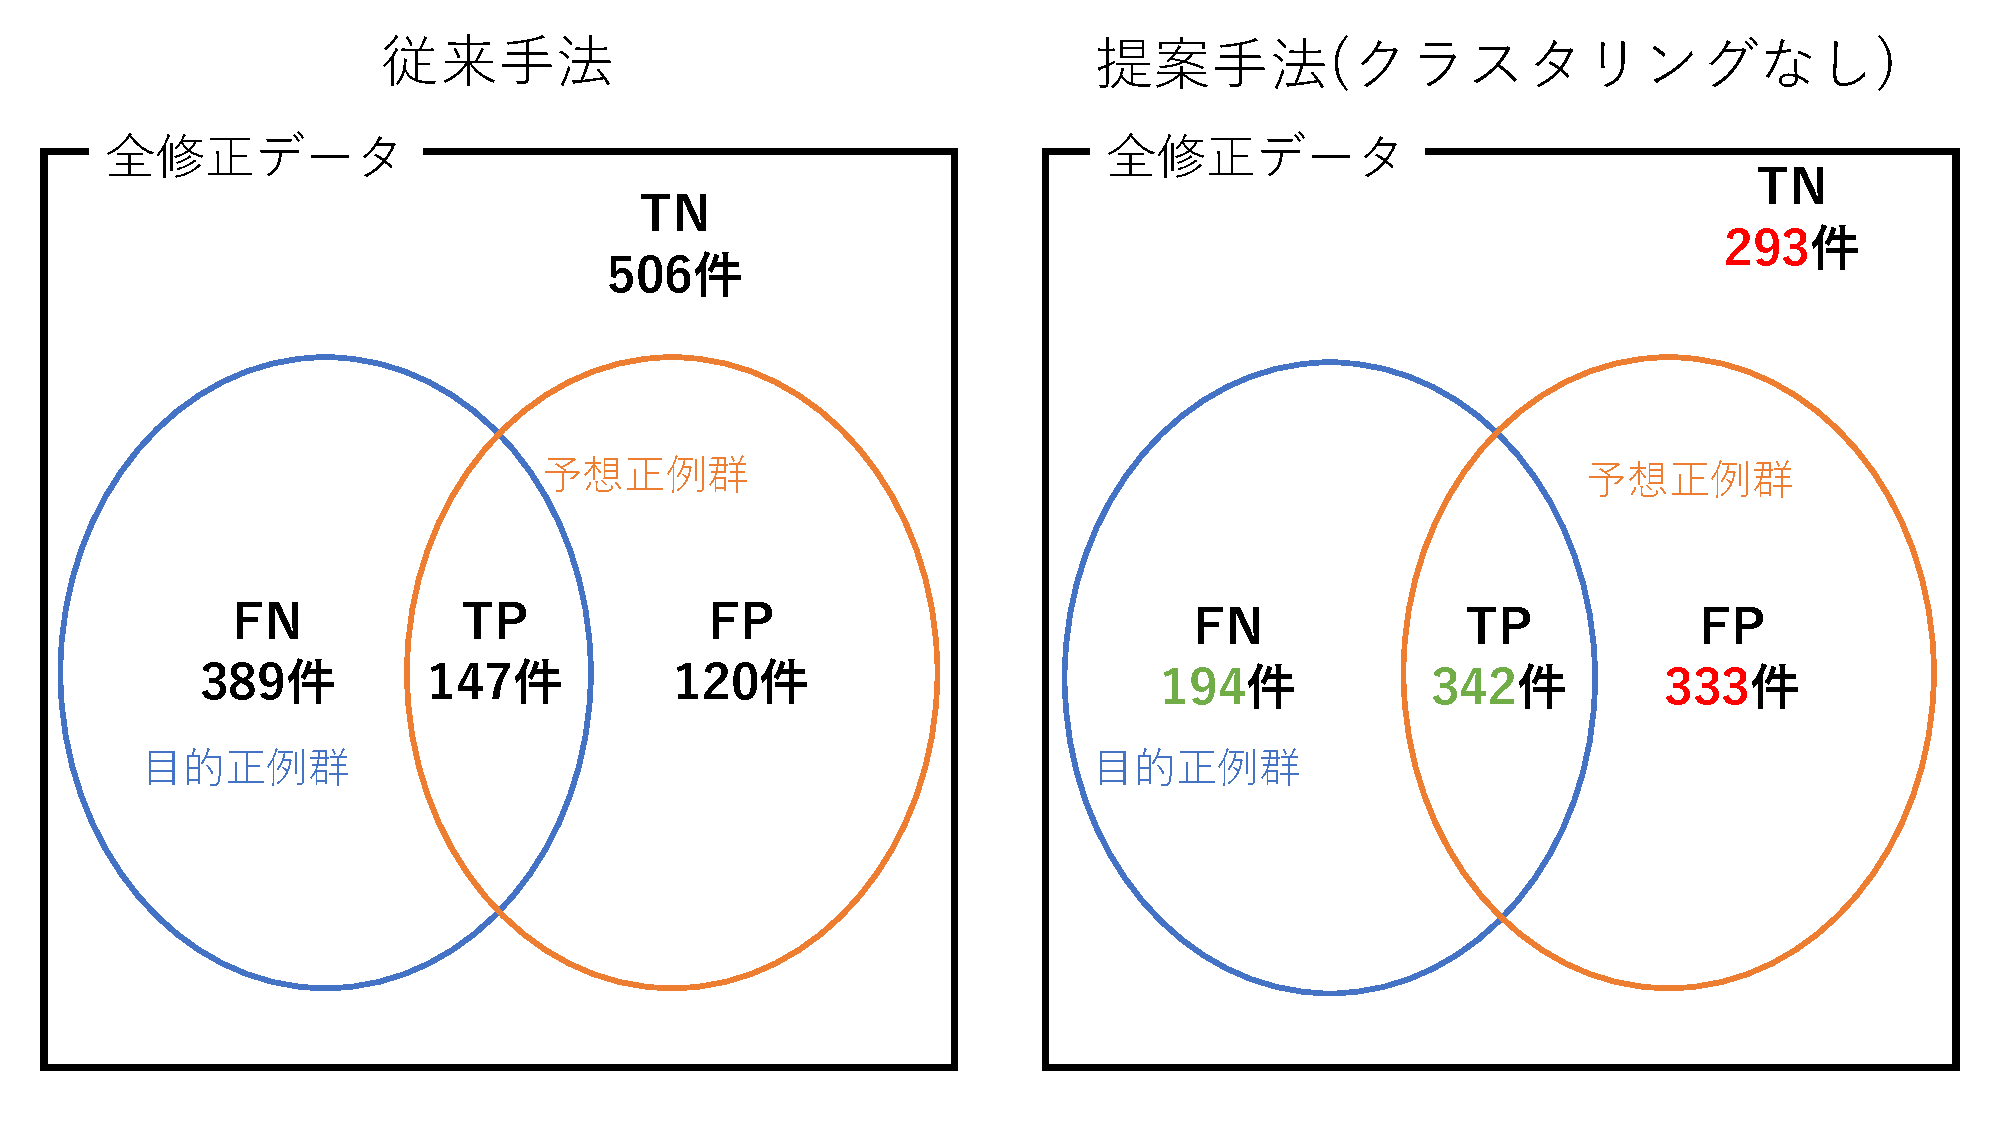
\includegraphics[width=1\linewidth]{Kameoka_fig/benzu-schema-salad.pdf}
	\caption{schema\_saladプロジェクトの手法ごとの予測結果のベン図}
	\label{fig:schema_salad}
\end{figure}

% \begin{figure}[bp]
% 	\centering
% 	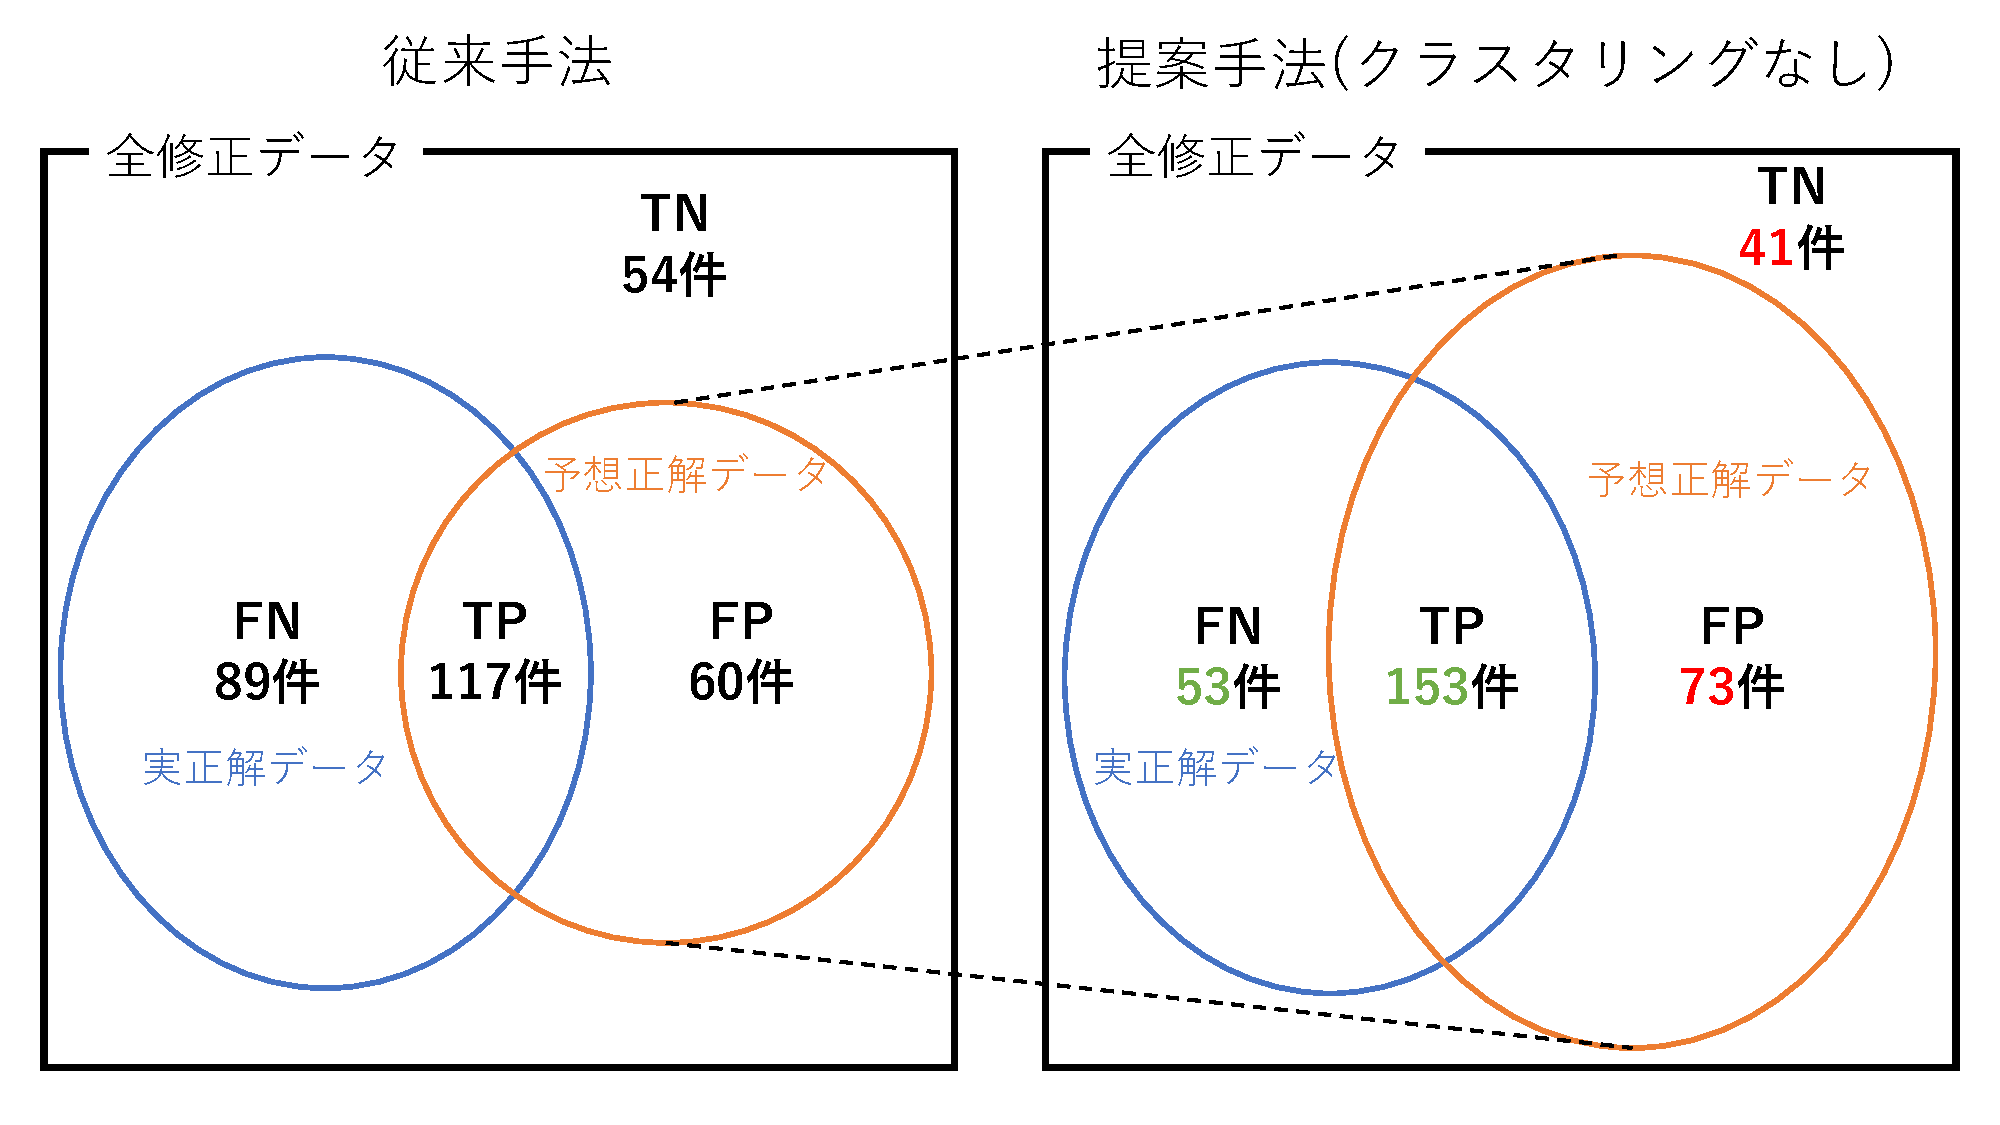
\includegraphics[width=1\linewidth]{Kameoka_fig/benzu-pyphi.pdf}
% 	\caption{pyphiプロジェクトの手法ごとの予測結果のベン図}
% 	\label{fig:pyphi}
% \end{figure}

\begin{figure}[bp]
	\centering
	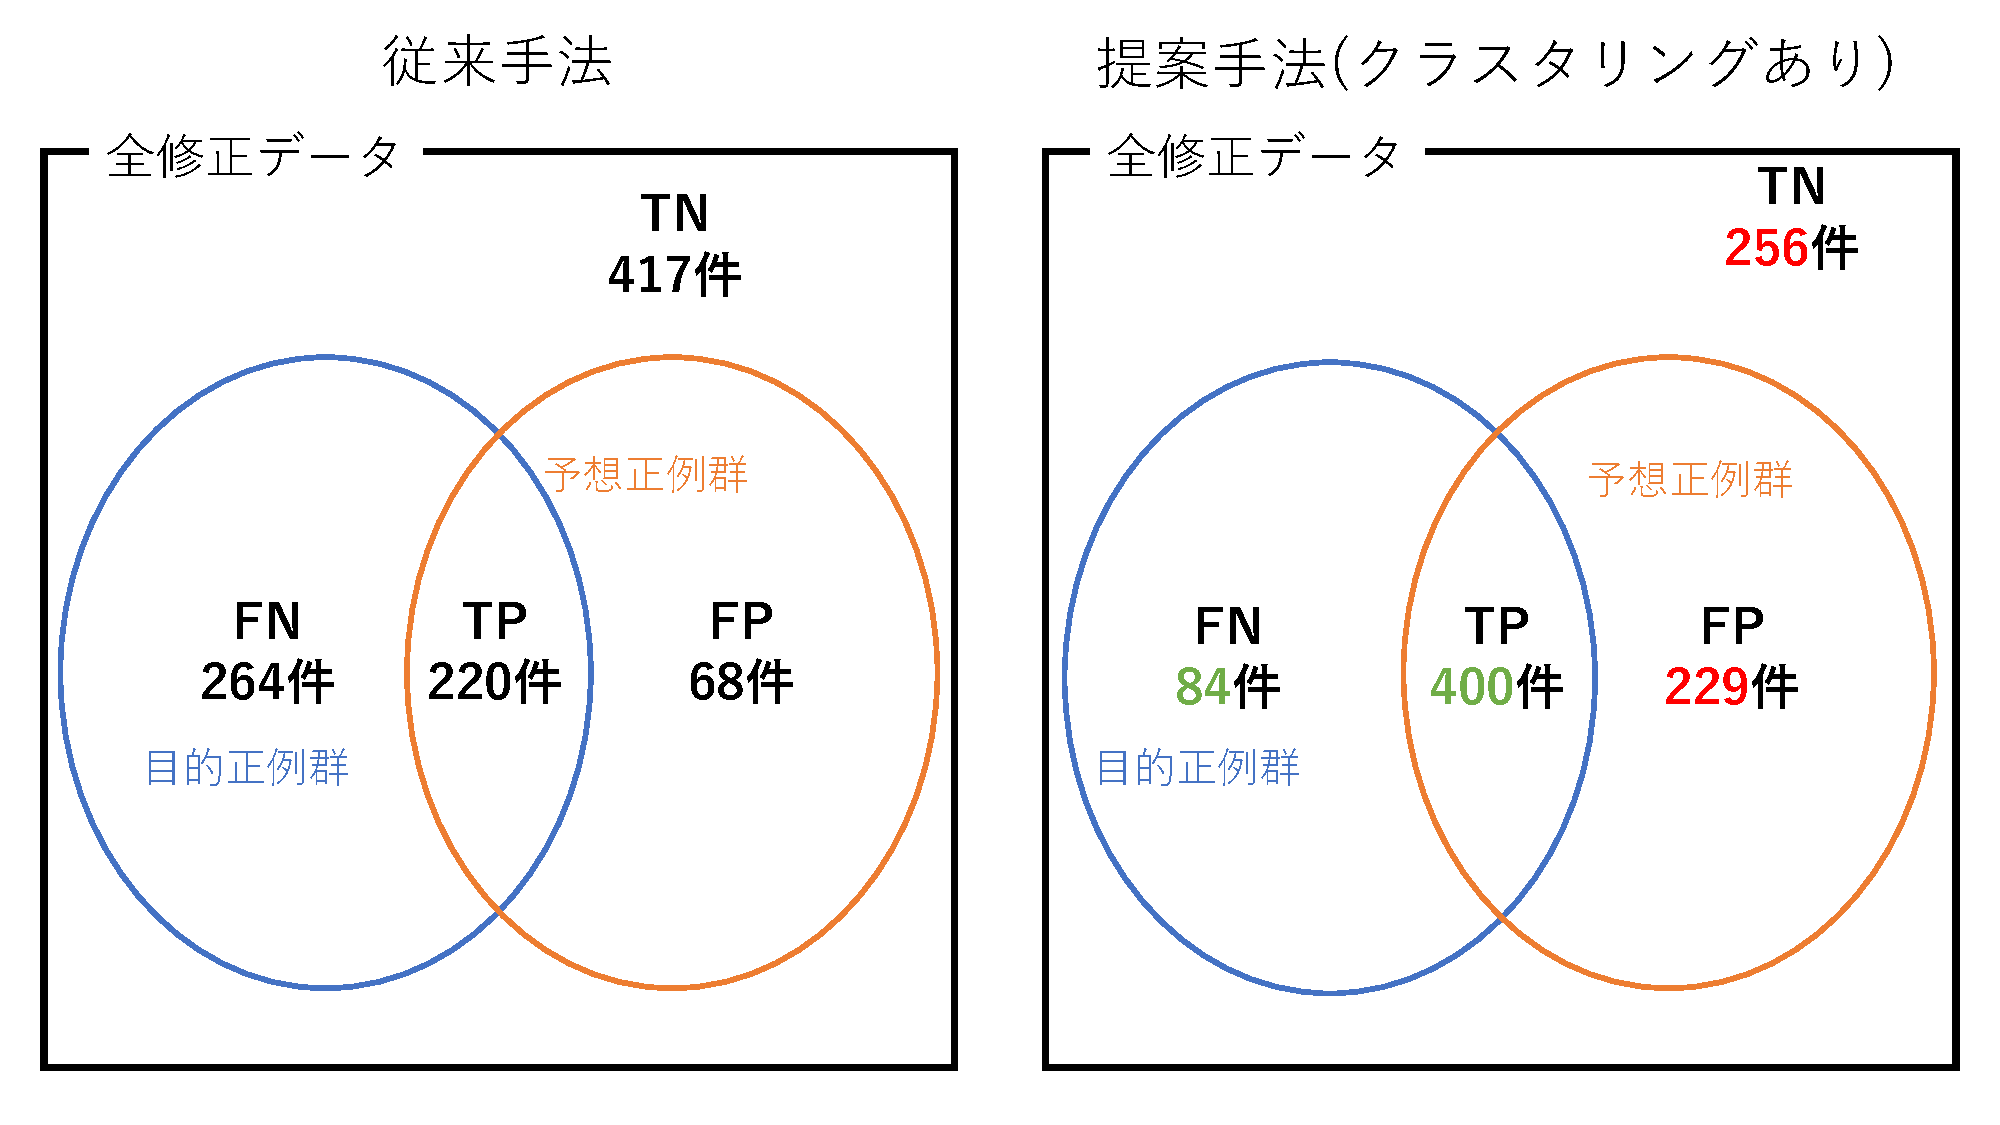
\includegraphics[width=1\linewidth]{Kameoka_fig/benzu-serverless-application-mode.pdf}
	\caption{serverless-application-modeプロジェクトの手法ごとの予測結果のベン図}
	\label{fig:serverless-application-mode}
\end{figure}

% \begin{figure}[bp]
% 	\centering
% 	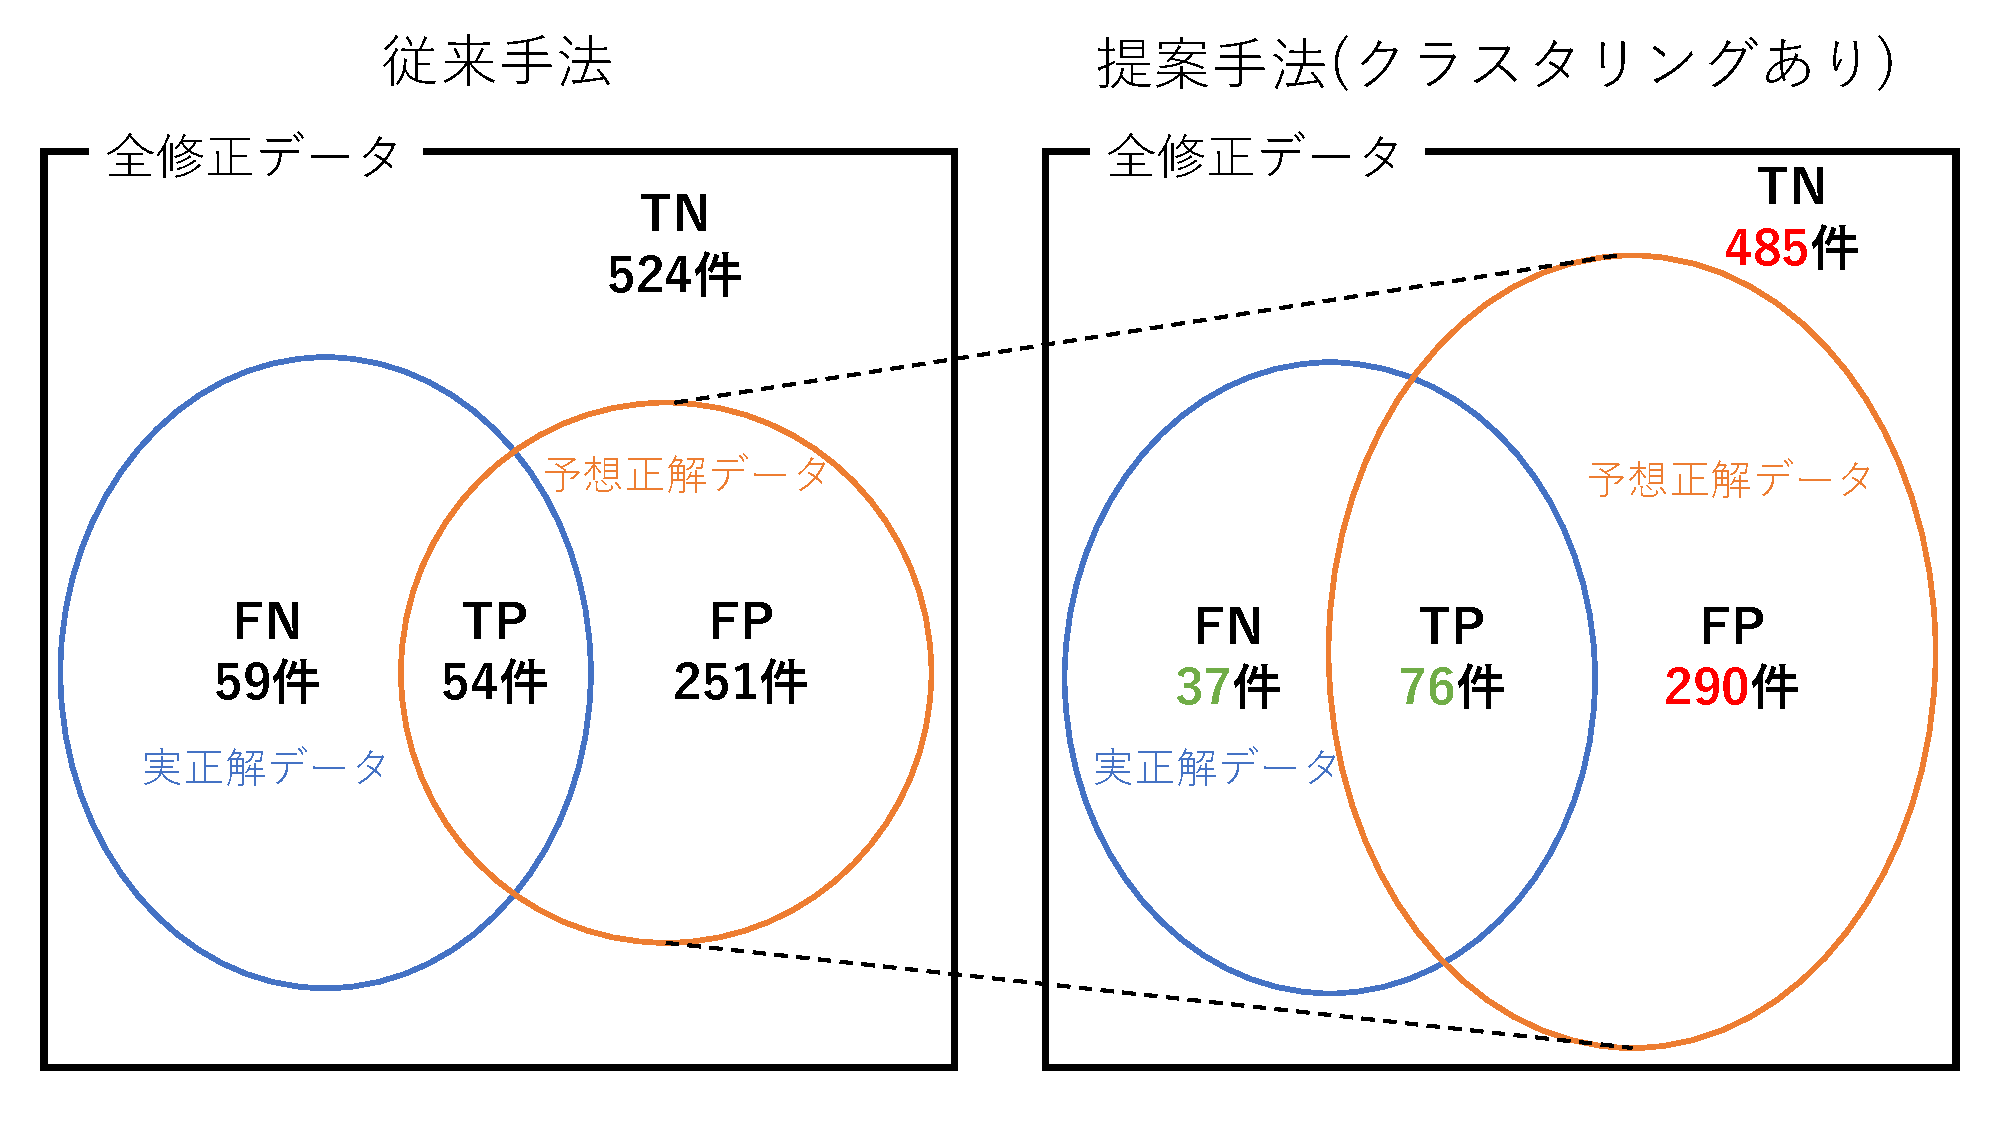
\includegraphics[width=1\linewidth]{Kameoka_fig/benzu-behave.pdf}
% 	\caption{behaveプロジェクトの手法ごとの予測結果のベン図}
% 	\label{fig:behave}
% \end{figure}

\begin{figure}[bp]
	\centering
	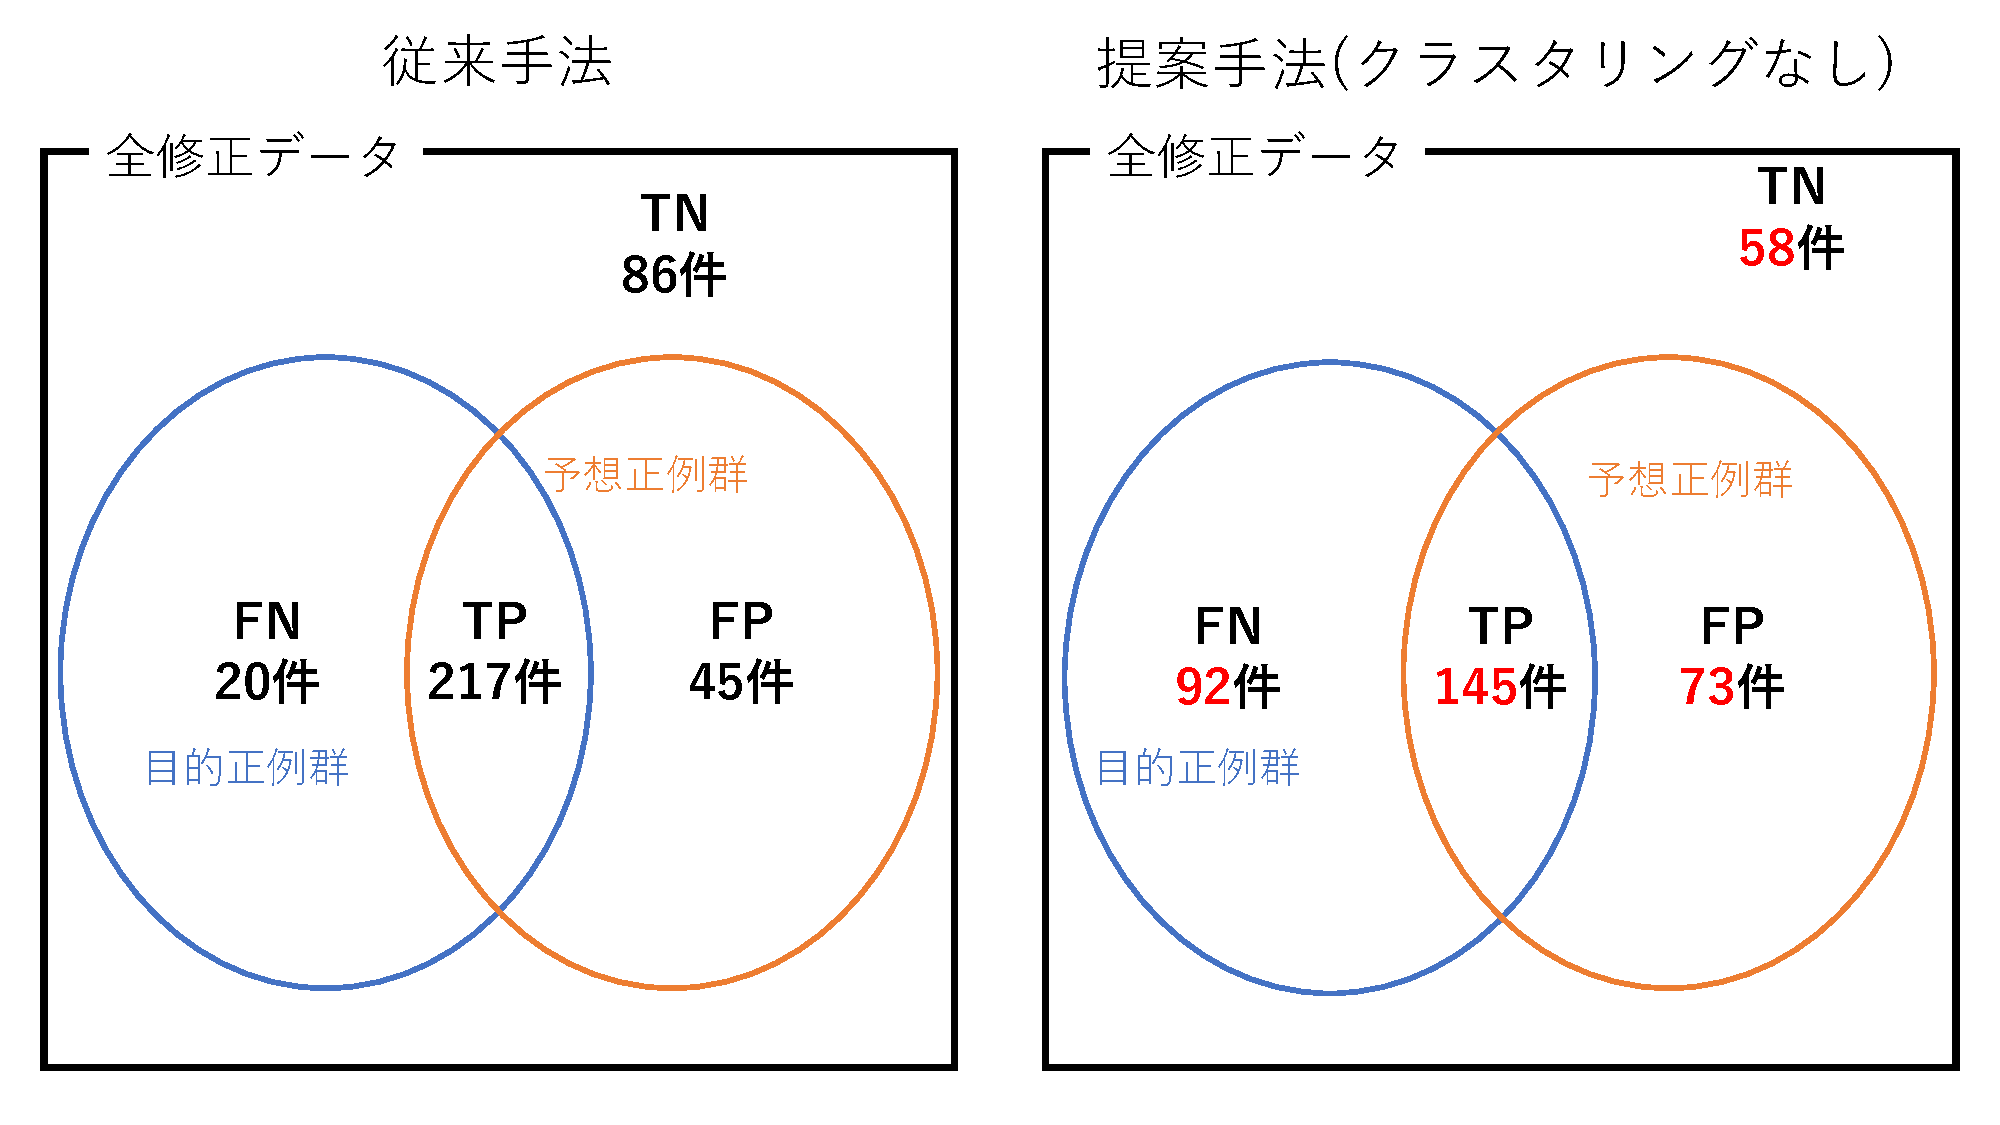
\includegraphics[width=1\linewidth]{Kameoka_fig/benzu-transitions.pdf}
	\caption{transitionsプロジェクトの手法ごとの予測結果のベン図}
	\label{fig:transitions}
\end{figure}
\begin{figure}[bp]

	\centering
	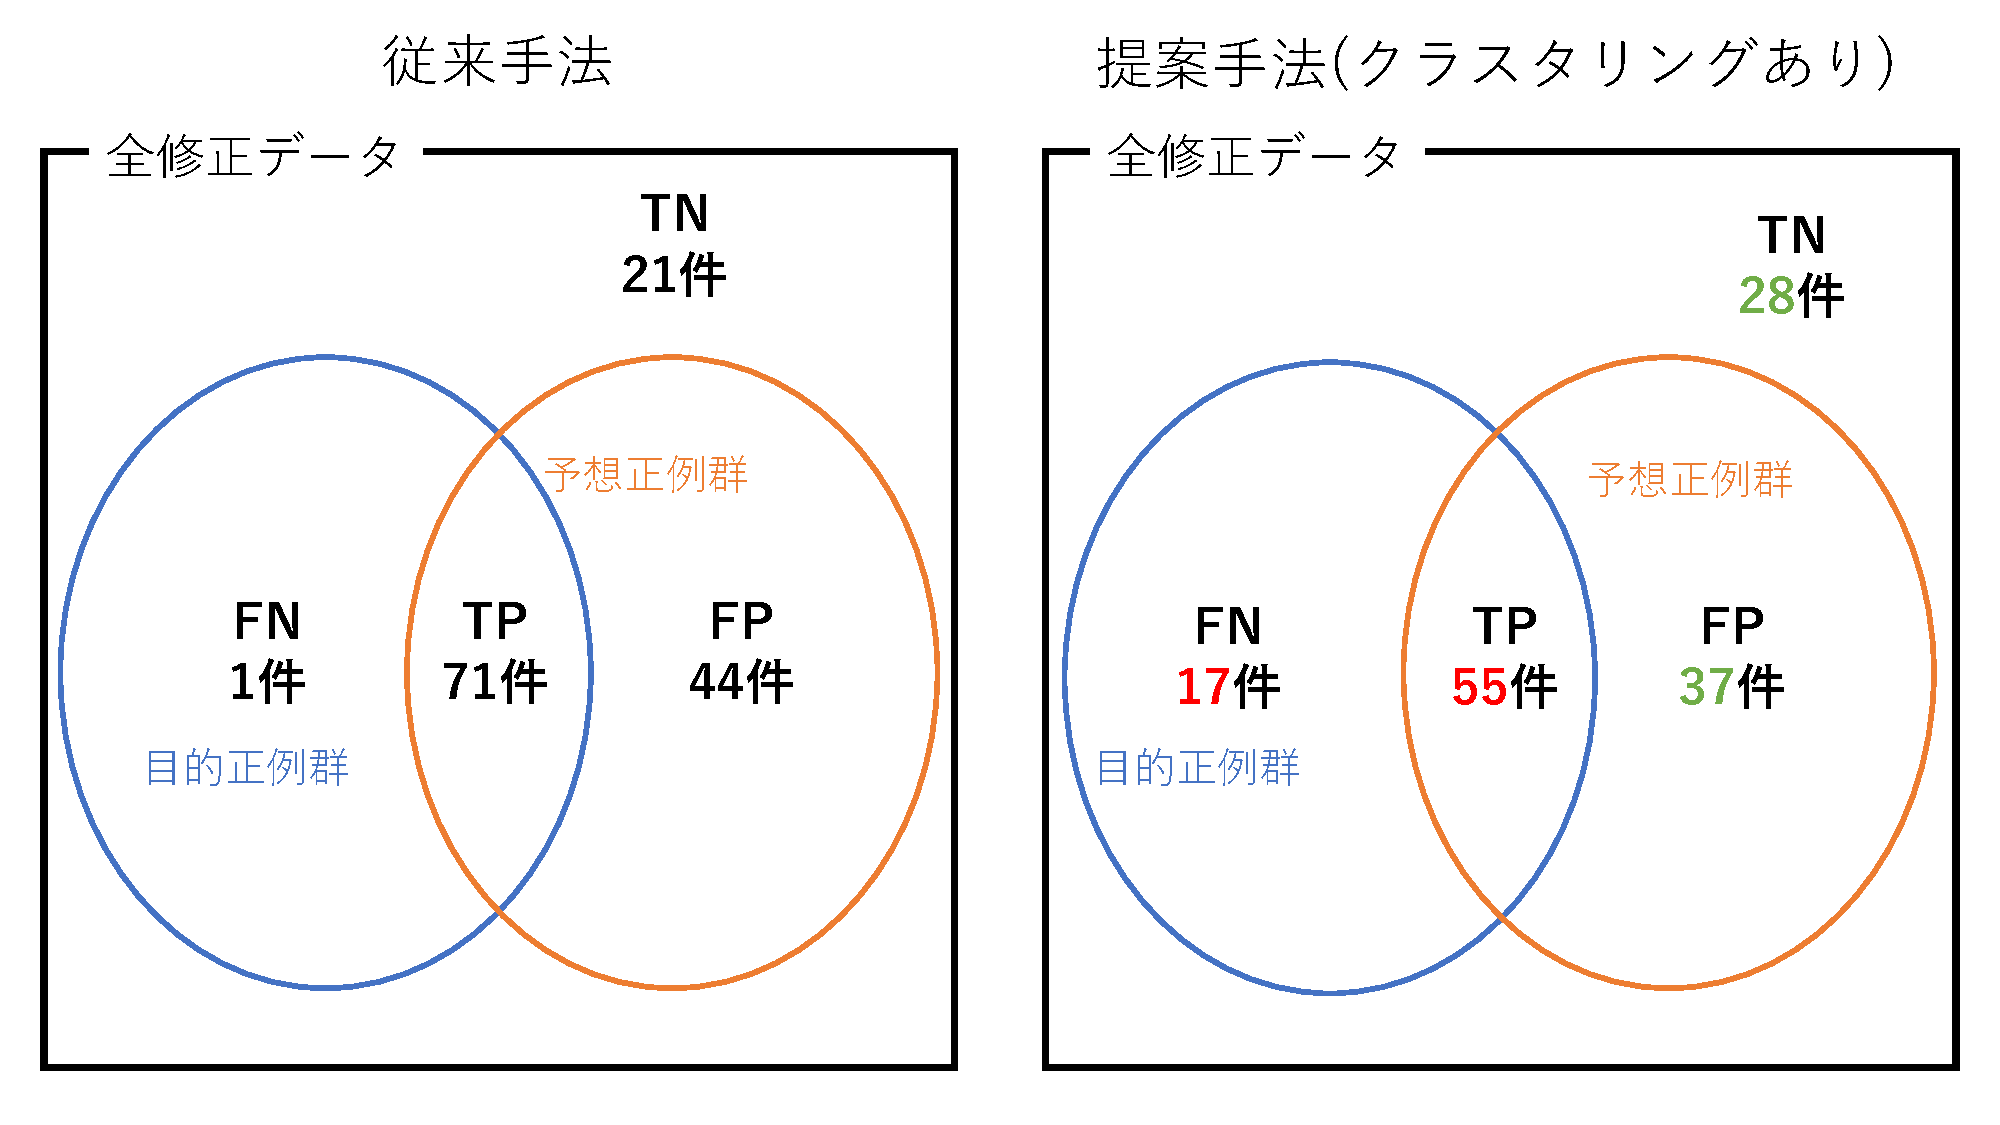
\includegraphics[width=1\linewidth]{Kameoka_fig/benzu-django-fsm.pdf}
	\caption{django-fsmプロジェクトの手法ごとの予測結果のベン図}
	\label{fig:django-fsm}
\end{figure}

RQ1の結果から,提案手法でデータセットを拡張したことによって,検出されたコーディング規約違反が修正されると予測した正例データが増加し,再現率が向上し,適合率が低下したことが示唆された.
本章では,従来手法と提案手法の具体的な予測結果について分析を行う.分析を行う対象として,RQ1において提案手法によって予測精度が向上したプロジェクトから選択して分析を行う.
ここで,プロジェクトを選択して分析を行うのは,従来手法と提案手法との予測結果の違いが顕著なプロジェクトを分析することで,提案手法の有効性を確認するためである.

表\ref{tab:log-super}はロジスティック回帰モデルを用いた提案手法によって再現率とF1値が共に向上したプロジェクトの予測結果から4プロジェクトを抜粋したものである.ロジスティック回帰モデルの結果を抜粋した理由としては,3種類のモデルの中で提案手法によって最も精度の改善が見られたからである.
1, 2行目のschema\_saladとserverless-application-modelプロジェクトは提案手法によって予測精度が向上し,3, 4行目のtransitionsとdjango-fsmプロジェクトは提案手法によって予測精度が低下した結果である.
表\ref{tab:log-super}に記載した提案手法によって予測精度が向上した2プロジェクト,提案手法によって予測精度が低下した2プロジェクトにおける修正予測結果について分析を行う.

図\ref{fig:schema_salad}から\ref{fig:django-fsm}に従来手法と提案手法(クラスタリングなし)または,従来手法と提案手法(クラスタリングあり)の予測結果をベン図にまとめる.図中のベン図は,プロジェクトで検出された全コーディング規約違反データの内,左側の円で囲われたものが目的変数の正例群を示し,右側の円は予測結果の正例群を示している.両方の円で囲まれた部分は実データと予測結果が共に正例であるためTPの違反修正箇所数を示し,左円のみに囲まれている部分は,予測できなかった正例であるためFNの修正箇所数を示し,右円のみに囲まれている部分は誤って正例と予測したためFPの修正箇所数を示し,どちらにも囲まれていない部分は,実際に修正されず予測でも修正されないと予測したためTNの修正箇所数を表している.

\subsection*{分析1 提案手法によって予測可能になったコーディング規約違反とは?}

図\ref{fig:schema_salad}のschema\_saladプロジェクトの予測結果から,提案手法(クラスタリングなし)によってFNが減少し,TPが増加しており,再現率が向上している.その一方で,FPが増加し ,TNが減少しているため,適合率が低下している.図\ref{fig:serverless-application-mode}に示すserverless-application-modelプロジェクトの予測結果も同様で,提案手法(クラスタリングあり)によってTPの増加とFNの減少によって予測精度の向上に影響を与えていることがわかる.
図\ref{fig:schema_salad}と図\ref{fig:serverless-application-mode}の結果は,データセットを拡張したことによって,予測できるようになった正例の数が増加したと同時に,誤って正例と予測した負例も増加した.schema\_saladプロジェクトでは,適合率が0.55から0.51(0.93倍)に低下し,再現率が0.27から0.64(2.37倍)に向上した.serverless-application-modeプロジェクトでは,適合率が0.76から0.64(0.84倍)に低下し,再現率が0.45から0.83(1.84倍)に向上した.
提案手法(クラスタリングなし)と提案手法(クラスタリングあり)の予測結果は従来手法からの再現率の上昇率が,適合率の低下率を上回る場合,適合率と再現率の両方を考慮した指標のF1値が向上する.
つまり,提案手法によって予測が可能となるコーディング規約違反は,従来手法でFNに位置していたコーディング規約違反が主である.



\subsection*{分析2 提案手法によって余剰に正例として予測したコーディング規約違反とは?}

図\ref{fig:transitions}と図\ref{fig:django-fsm}に提案手法によって予測精度が低下した場合の予測結果の内訳をベン図に示す.図\ref{fig:transitions}は提案手法(クラスタリングなし)によって従来手法よりTPとTNがともに減少し,FPとFNがともに増加している結果である.
transitionsプロジェクトは従来手法によってTPが217件から145件に減少し,TNも86件から58件に低下している.
これは,従来手法によってプロジェクトの修正の特徴をとらえた修正予測ができていたものを提案手法によって,汎化したモデルを用いたため,すべての指標において予測精度が低下したためと考えられる.

図\ref{fig:django-fsm}は提案手法(クラスタリングあり)によって予測精度が低下したdjango-fsmプロジェクトの予測結果を示す.transitionsプロジェクトと同様に従来手法より予測精度が低下しているが,django-fsmプロジェクトは提案手法によってTNが増加し,FPが減少しており予測精度の向上につながる変化も見られるが,TPの減少とFNの増加のほうが顕著であり予測精度が低下したことがわかる.
よって,transitionsやdjango-fsmのようなプロジェクトの場合では従来手法のように単一プロジェクトの規約修正履歴のみを学習し,予測を行う方が効果的であることがわかる.
分析2の結果から,提案手法によって従来手法より適合率が低下するのは,複数プロジェクトのデータを学習したことによって,TPとして予測できていたものをFNと予想してしまうためである.

\subsection{結果のまとめ}

提案手法(クラスタリングなし),提案手法(クラスタリングあり)によって予測精度が向上しているプロジェクトでは,データセットを拡張したことによってTPが増加,FNが減少したことによる再現率の向上と,それに伴うF1値の向上によって従来手法を上回る予測精度でコーディング規約違反の修正予測が可能となった.しかし,従来手法によって高い精度で予測できているものは,提案手法によってTPが減少する場合や,FPがTPの増加より上回って増加してしまう場合は再現率が低下しF1値も低下する.

\chapter{考察}\label{chap:consideration}

\section{RQの結果からなぜ提案手法によって再現率が向上したのか}\label{kosatu}

RQ1の結果では提案手法の再現率が従来手法に比べて向上し,F1値も向上することが明らかになった.
その理由としては,RQ2の結果から,従来手法は正例として予測できなかったコーディング規約違反の修正予測を提案手法によって予測が可能になったためである.
また,提案手法を用いることによって,従来手法では予測ができなかった正例を正しく予想できるようになったのは,複数プロジェクトを学習し,単一プロジェクトでは十分に学習できなかったコーディング規約について学習ができたためであると考えられる.
本研究ではPylintのコーディング規約の種類はone-hotベクトル化して説明変数として利用している.そのため,単一プロジェクトにおいて低頻度でしか発生しないコーディング規約違反が修正されたデータが学習データにある場合その規約に過剰な重みが与えられた結果として,誤った予測をしてしまうことが考えられる.コーディング規約を種類ごとにone-hotベクトル化している点においては,単一プロジェクトで頻出しているコーディング規約違反があった場合に,単一プロジェクトで的確な重みづけができていたものを,複数プロジェクトのコーディング規約が結合されたことによって,重みづけが汎化され予測精度に悪影響を及ぼすことが考えられる.

本研究では,コーディング規約の修正予測において,複数プロジェクトの開発データを学習に用いることによって予測精度が向上するプロジェクトが68プロジェクトの半数程度存在することが明らかになった.今後提案手法が有効に働くプロジェクトの特徴を明らかにすることによって,本研究の提案手法を適用する場面が明確になると考えられる.

\section{提案手法(クラスタリングあり)の有効性とは}

\begin{table}[th]
    \centering
    \caption{クラスタごとの予測結果の分析}
    \label{tab:cluster}
    \vspace{3mm}
    \scalebox{0.80}{
        \begin{tabular}{l|p{3em}|p{3em}|p{3em}|p{3em}|p{3em}|p{3em}|p{3em}|p{3em}|p{3em}|p{3em}}
        \hline
        cluster & \hfill 01 & \hfill 02 & \hfill 03 & \hfill 04 & \hfill 05 & \hfill 06 & \hfill 07 & \hfill 08 & \hfill 09 & \hfill 10 \\ \hline
        適合率 & \hfill 0.34 & \hfill 0.09 & \hfill 0.57 & \hfill 0.47 & \hfill 0.51 & \hfill nan & \hfill 0.00 & \hfill nan & \hfill nan & \hfill nan \\
        再現率 & \hfill 0.64 & \hfill 0.59 & \hfill 0.39 & \hfill 0.83 & \hfill 0.72 & \hfill nan & \hfill 0.00 & \hfill nan & \hfill nan & \hfill nan \\ 
        F1値 & \hfill 0.44 & \hfill 0.16 & \hfill 0.46 & \hfill 0.60 & \hfill 0.60 & \hfill nan & \hfill nan & \hfill nan & \hfill nan & \hfill nan \\ \hline
        テストデータ数 & \hfill 18,368 & \hfill 259 & \hfill 82 & \hfill 2,129 & \hfill 4,719 & \hfill 0 & \hfill 86 & \hfill 1 & \hfill 495 & \hfill 0 \\ \hline
        \end{tabular}
    }
\end{table}

提案手法として,複数プロジェクトのデータを結合した後にクラスタリングを行い,各クラスタごとにロジスティック回帰予測モデルを作成し予測を行った.クラスタリングによる予測精度の変化を分析するために,各クラスタごとの予測精度を算出した.表\ref{tab:cluster}に,各クラスタごとの予測精度を示す.表の最下列は各クラスタに分類されたテストデータ数を示している.表からわかるようにcluster06とcluster10にはテストデータが存在せず,cluster01,cluster04,cluster05に多くのデータが集まっている.表中の`nan'は予測結果をすべて負例として予想した場合に適合率,再現率.F1値が計算できずに代入される.
クラスタごとの予測結果で最もF1値が高いのはcluster04,cluster05の0.60である.また,cluster06以降では違反修正データの有無に関わらず修正予測ができていない.各クラスタごとに各評価指標の値に違いが見られるため,総違反修正データのクラスタリングが予測精度に影響を与えていることがわかる.また,cluster04,cluster05のデータ数は2,129と4,719であり,cluster01はクラスタに含まれるデータ数が過多であり,cluster02とcluster03はデータ数が過小であると考えられる.

各クラスタごとの予測精度から,クラスタリングにより抜粋された説明変数のみ学習する提案手法(クラスタリングあり)は,クラスタごとに予測精度が異なり,クラスタに含まれるデータ数が2,129と4,719の際に最大のF1値を確認したため,各クラスタに含まれるデータ数をcluster04,cluster05に近づけるようにクラスタリングを行うことによって,更なる予測精度の向上を見込むことができる.


\chapter{妥当性への脅威}\label{chap:heuristic}
\section{内的妥当性}

% 本研究で利用したデータセットは,プロジェクトごとの規約修正履歴の期間は統一して収集しているが,複数プロジェクトを結合して学習した場合には予測地点では得られない他プロジェクトの未来のデータを学習している.複数プロジェクトのデータを学習し,予測する際にも時系列を考慮することは今後の課題である.

目的変数の計測において,規約違反しているコードが修正された場合のみ正例として扱い,削除された場合は,修正されたわけではないため本研究では負例として扱っている.しかし,コーディング規約違反の中には該当部分を削除することによっても解消するものがあるため,本来正例として扱うべきケースを負例として計測してしまっていることがある.
また,目的変数の計測は一様に最終リビジョンにおいて,コーディング規約違反が修正されたか否かで計測しており,違反の発生地点は考慮していない.つまり,最終リビジョンの一つ前のリビジョンで発生した違反と,最初のリビジョンで発生した違反を同等に扱っているため,最終リビジョンに近いほど修正までの猶予が短いことを考慮していない.

本研究では2値分類機械学習アルゴリズムとして,ロジスティック回帰,RandomForest,SVMの3種類のアルゴリズムを用いて検出されたコーディング規約違反の修正予測を行った.結果として,RandomForestが最も高い精度で予測し,SVMが最も低い精度での予測結果となった.
本研究で用いた3種類の機械学習アルゴリズム以外にも、より正確な予測を可能にするアルゴリズムが存在する可能性がある.
それぞれのパラメータの更新回数である,イテレーション回数を10,000に設定したが,データサイズが大きいプロジェクトではモデルが収束しないことが確認された.モデルが収束しない場面も確認されたが,本研究で主に用いた実験環境とは別の環境で,複数回実行した場合でも予測結果に変化はなかったので,モデルが収束しない問題に関しては,本研究の結果に対して大きな影響を与える可能性は低い.

提案手法で説明変数の階層的クラスタリングを行う際に,クラスタ間の連結法にはWard法を用い,距離の測定にはユークリッド距離を用いた.連結法や距離の測定方法にはPython言語のライブラリであるsklearnのAgglomerativeClusteringパッケージ\footnote{sklearn.cluster.AgglomerativeClustering: \\ \url{https://scikit-learn.org/stable/modules/generated/sklearn.cluster.AgglomerativeClustering.html}}のデフォルト値を使用している.階層的クラスタリングする際の連結法や距離の測定方法を変えることによって,各データが属するクラスタが変化すると考えられるが,本研究でのクラスタリングの結果では,大多数のデータが集まるクラスタと,そうでないクラスタに二極化したため,連結法と距離の測定方法による結果への影響は小さいと考えられる.

\section{外的妥当性}

本研究ではケーススタディとしてPython言語を主な開発言語としたプロジェクト68件の規約修正履歴を収集して検証を行った.
また,プロジェクト数をさらに拡張した場合や,対象とするプロジェクトや期間を変更した場合に予測精度が変化することが示唆される.
対象言語をPython以外の言語を対象とした場合予測結果が変化することが示唆される.
しかし,本研究で使用したデータセットは68プロジェクトでプロジェクトごとのデータ数が中央値で500.5件のデータ数を含んでいるので,更なるデータサイズの拡張による予測精度への影響は低いと考えられる.

%-----------------------------------prev
% 本研究ではケーススタディとして10プロジェクト分のデータを学習し予測を行ったが,データセットを拡張することによって正例が増加し予測性能が向上することも示唆されるが,一方で,学習データ増加により各クラスタで作成したモデルが汎化することも考えられる.今後は,プロジェクト数,クラスタ数の適性についても検討する.
%-----------------------------------

\chapter{おわりに}\label{chap:end}

本研究では,静的解析ツールによってソースコード中に含まれるコーディング規約違反を検出した結果から,修正すべき違反か否かに分類するタスクにおいて予測対象プロジェクト以外の開発データも予測モデルの学習に用いた場合の予測結果への影響を調査した.結果として,ロジスティック回帰モデル,RandomForestモデル,SVMモデルの3種類のモデル構築手法において,従来手法である予測対象プロジェクトの過去の規約修正履歴のみを学習した場合が,提案手法より多いプロジェクトで高いF1値で修正予測が可能であった.しかし,予測対象プロジェクト以外の開発データも学習する提案手法(クラスタリングなし),提案手法(クラスタリングあり)によって検証に使用した68プロジェクトの1/4程度ずつのプロジェクトでF1値の向上を確認した.
F1値が向上した理由として,データセットを拡張したことによるTPの増加とそれに伴うFNの減少によって予測精度が向上したことが明らかになった.

本研究において複数プロジェクトを学習に用いる提案手法によって予測精度が向上するプロジェクトを確認することができたので,精度が向上するプロジェクトの特徴を分析し,提案手法が有効に働くプロジェクトに対してのみ複数プロジェクトの開発データを学習するように,適用プロジェクトを分類することにより,本研究の提案手法がより有用に活用できることが示唆される.
% 適用プロジェクトの分類は単純にプロジェクトが保有するデータ数やメトリクスでは判断ができず,更なる分析が必要である.


%-----------------------------------prev
% 本研究では,静的解析ツールによって大量に検出されるコーディング規約に違反しているコード断片の中から,優先して修正すべき違反の予測を,複数プロジェクトのデータを結合し,類似性に基づいてクラスタリングしたデータセットを用いることによる予測精度への影響を明らかにした.検証の結果,予測精度だけを見れば,単一プロジェクトのデータだけを用いて学習するほうが予測に効果的であった.今後は考察でも述べたように,多くのデータを保有するクラスタをさらに分割することや,データ数の少ないクラスタ同士の結合によって修正予測精度の向上を目指し,複数プロジェクトのデータを機械学習モデルに学習させる手法の有効性を明らかにする.
%-----------------------------------

\chapter*{謝辞}\label{chap:thanks}

研究活動に取り組むにあたって多くの方々に御指導,御協力を賜りました.ここに御世話になった方々への感謝の意を記させていただきます.はじめに,指導教員である和歌山大学システム工学部伊原彰紀准教授に対し,厚く御礼申し上げます.研究室に配属して以来,研究方針についての相談,論文執筆,発表資料制作など多くの時間を割いて御指導をしていただきました.特に学会発表の際には,夜分にもかかわらずご対応いただき,無事発表を行うことができました.先生の御尽力に敬意を表し,心より感謝いたします.

次に,和歌山大学システム工学研究科を修了された南雄太氏並びに,和歌山大学システム工学研究科大森楓己氏には,研究において多くの御指導,御協力,御助言をしていただきました.お忙しい中,研究内容の相談や,論文執筆,実装方法についての支援だけでなく,発表資料制作についても多大なるご協力を賜りました.心より感謝いたします.

また,和歌山大学ソーシャルソフトウェア工学研究室の方々には,研究に関する客観的な御意見や御指摘を常日頃からかず多くいただきました.研究活動の他にも,研究室での生活においても,大変お世話になりました.特に切磋琢磨し互いに高めあうことができた同期がいたことが,研究生活において大きな支えとなりました.心より感謝いたします.

%-----------------------------------prev
% 研究を進めるにあたり多くの方々に,御指導,御協力,御支援を賜りました.ここに御世話 になった方々への感謝の意を記させていただきます.はじめに,指導教員である和歌山大学シス テム工学部伊原彰紀講師に対し,厚く御礼申し上げます.研究室配属以降,研究内容の議論,論 文執筆,発表資料制作など多くの時間を割いて御指導をしていただきました.特に,学会発表の 機会をいただいたことで,研究に対する視野を広げることができました.先生の御尽力に敬意を 表し,心より感謝いたします.

% 次に,和歌山大学システム工学研究科才木一也氏には,研究において多くの御指導,御協力,御 助言をしていただきました.研究内容の議論のため,お忙しい中,平時よりお気遣いいただきま した.特に,分析手法や実装方法,発表練習など多くの御指導を賜りました.心より感謝いたし ます.

% また,和歌山大学ソーシャルソフトウェア工学研究室の方々には,研究に関する客観的な御意 見や御協力を常日頃から数多くいただきました.研究活動だけでなく,大学生活においても大変 お世話になりました.研究室の方々と交流を深めたり,切磋琢磨し合う同期がいたことは,研究 活動を進める上で支えとなりました.心より感謝いたします.最後になりましたが,日頃から暖 かく見守り,支えてくださった家族には心より感謝いたします
%-----------------------------------

%%%%%%%%%%%%%%%%%%%%%%%%%%%%%%%%%%%%%%%%%%%%%%%%%%%%%%%%%%%%%%%%%%%%%%%%

%%
%% 謝辞
%%
%% \begin{acknowledgements}
%% 感謝します.
%% \end{acknowledgements}

%%%%%%%%%%%%%%%%%%%%%%%%%%%%%%%%%%%%%%%%%%%%%%%%%%%%%%%%%%%%%%%%%%%%%%%%

%%
%% 参考文献
%%
\bibliographystyle{junsrt}
\bibliography{Kameoka}

%%%%%%%%%%%%%%%%%%%%%%%%%%%%%%%%%%%%%%%%%%%%%%%%%%%%%%%%%%%%%%%%%%%%%%%%

%%
%% 付録
%%
% \appendix
% 
% \chapter{サンプルプログラム}
% 
% プログラムリストや実行結果など,本論を補足する上で必要と思われるものが
% あれば付録として付ける.
% 
% {
% \footnotesize
% \begin{verbatim}
% #include <stdio.h>
% int main(void)
% {
%     printf("Hello, World!\n");
%     return 0;
% }
% \end{verbatim}
% }

%%%%%%%%%%%%%%%%%%%%%%%%%%%%%%%%%%%%%%%%%%%%%%%%%%%%%%%%%%%%%%%%%%%%%%%%

\end{document}
